\documentclass{article}

\usepackage[utf8]{inputenc}
\usepackage[english]{babel}
\usepackage{authblk}
\usepackage{amssymb,amsmath,amsthm,twoopt,xargs,mathtools}
\usepackage{times,dsfont,ifthen}
\usepackage{fancyhdr,xcolor,breakcites,booktabs}

\title{Backward importance sampling for online estimation of models with intractable likelihood}
\date{}


\author[$\dag\,\amalg$]{Alice Martin}
\author[$\wr$]{Marie-Pierre \'Etienne}
\author[$\star$]{Pierre Gloaguen}
\author[$\dag$]{Sylvain Le Corff}
\author[$\ddag$]{Jimmy Olsson}

\affil[$\dag$]{{\small Samovar, T\'el\'ecom SudParis, d\'epartement CITI, TIPIC, Institut Polytechnique de Paris, Palaiseau.}}
\affil[$\wr$]{{\small Agrocampus Ouest, CNRS, IRMAR - UMR 6625, F-35000 Rennes.}}
\affil[$\amalg$]{{\small CMAP, \'Ecole Polytechnique, Institut Polytechnique de Paris, Palaiseau.}}
\affil[$\star$]{{\small AgroParisTech, UMR MIA 518.}}
\affil[$\ddag$]{{\small Department of Mathematics, KTH Royal Institute of Technology, Stockholm.}}


\lhead{}
\rhead{Backward importance sampling}


\usepackage{geometry}
\pagestyle{fancy}

\newcommand{\gpeUB}{\overline{m}_{\parvec}}
\newcommand{\gpeLB}{\underline{m}_{\parvec}}

\def\dimX{d}
\def\dimY{m}
%\def\Xset{\mathsf{X}}
\def\Xset{\mathbb{R}^d}
\def\Yset{\mathsf{Y}}
\newcommand{\mk}{\kernel{G}}
\newcommand{\hk}{\kernel{Q}}
\newcommand{\md}[1]{g_{#1}}
\newcommand{\SmoothFigSize}{0.27}

\newcommand{\logllh}[1]{\ell_{#1}}
\newcommand{\llh}[1]{\mathsf{L}_{#1}}
\newcommand{\testf}{\mathsf{h}}

\newcommandx\filtderiv[2][1=]{
\ifthenelse{\equal{#1}{}}
	{\eta_{#2}}
	{\eta_{#2}^\N}
}
\newcommand{\pred}[1]{\pi_{#1}}
\newcommand{\parvec}{\theta}
\newcommand{\parspace}{\Theta}
\newcommand{\tstatletter}{\kernel{T}}
\newcommand{\retrok}{\kernel{D}}
\newcommandx\tstat[2][1=]{
\ifthenelse{\equal{#1}{}}
	{\tstatletter_{#2}}
	{\tau_{#2}^{#1}}
}
\newcommandx\tstathat[2][1=]{
\ifthenelse{\equal{#1}{}}
	{\tstatletter_{#2}}
	{\widehat{\tau}_{#2}^{#1}}
}
\newcommand{\af}[1]{h_{#1}} 
\newcommand{\deriv}{\nabla_{\parvec}}

\newcommand{\kernel}[1]{\mathbf{#1}}
\newcommand{\bmf}[1]{\set{F}(#1)}
\newcommand{\set}[1]{\mathsf{#1}}

\newcommandx{\bk}[2][1=]{ 
\ifthenelse{\equal{#1}{}}
{\overleftarrow{\kernel{Q}}_{#2}}
{\overleftarrow{\kernel{Q}}_{#2}^{#1}}
}

\newcommandx{\bkhat}[2][1=]{ 
\ifthenelse{\equal{#1}{}}
{\widehat{\kernel{Q}}_{#2}}
{\widehat{\kernel{Q}}_{#2}^{#1}}
}

\newcommand{\lk}{\kernel{L}}
\newcommand{\idop}{\operatorname{id}}
\newcommand{\hd}[1]{q_{#1}} 
\newcommand{\hdhat}[1]{\widehat{q}_{#1}} 


\newcommand{\addf}[1]{\termletter_{#1}}
\newcommand{\addfc}[1]{\underline{\termletter}_{#1}}
\newcommand{\adds}[1]{\af{#1}}
\newcommand{\term}[1]{\termletter_{#1}}
\newcommand{\termletter}{\tilde{h}}
\newcommand{\N}{N}
\newcommand{\partpred}[1]{\pi_{#1}^\N}
\newcommand{\tstattil}[2]{\tilde{\tau}_{#2}^{#1}}
\newcommandx{\K}[1][1=]{
\ifthenelse{\equal{#1}{}}{{\kletter}}{{\widetilde{\N}^{#1}}}}
\newcommand{\hkup}{\bar{\varepsilon}}
\newcommand{\bi}[3]{J_{#1}^{(#2, #3)}}
\newcommand{\bihat}[3]{\widehat{J}_{#1}^{(#2, #3)}}

\newcommand{\kletter}{\widetilde{\N}}

\def\sigmaX{\mathcal{X}}
\def\sigmaY{\mathcal{Y}}
\def\1{\mathds{1}}
\def\pE{\mathbb{E}}
\def\pP{\mathbb{P}}
\def\plim{\overset{\pP}{\longrightarrow}}
\def\dlim{\Longrightarrow}
\def\gauss{\mathcal{N}}


\newcommand{\esssup}[2][]
{\ifthenelse{\equal{#1}{}}{\left\| #2 \right\|_\infty}{\left\| #2 \right\|^2_{\infty}}}


\newcommand{\swght}[2]{\ensuremath{\omega_{#1}^{#2}}}

\newtheorem{assumptionA}{\textbf{A}\hspace{-3pt}}
\newcommand{\rset}{\ensuremath{\mathbb{R}}}
\newcommand{\iid}{i.i.d.}

\newcommand{\smwght}[3]{\tilde{\omega}_{#1|#2}^{#3}}
\newcommand{\smwghtfunc}[2]{\tilde{\omega}_{#1|#2}}

\newcommand{\smpart}[3]{\ensuremath{\tilde{\xi}_{#1|#2}^{#3}}}
\def\aux{{\scriptstyle{\mathrm{aux}}}}
\newcommand{\bdm}{\mathsf{TwoFilt}_{bdm}}
\newcommand{\fwt}{\mathsf{TwoFilt}_{fwt}}

\newcommand{\kiss}[3][]
{\ifthenelse{\equal{#1}{}}{r_{#2|#3}}
{\ifthenelse{\equal{#1}{fully}}{r^{\star}_{#2|#3}}
{\ifthenelse{\equal{#1}{smooth}}{\tilde{r}_{#2|#3}}{\mathrm{erreur}}}}}

\newcommand{\chunk}[4][]%
{\ifthenelse{\equal{#1}{}}{\ensuremath{{#2}_{#3:#4}}}{\ensuremath{#2^#1}_{#3:#4}}
}

\newcommand{\kissforward}[3][]
{\ifthenelse{\equal{#1}{}}{p_{#2}}
{\ifthenelse{\equal{#1}{fully}}{p^{\star}_{#2}}
{\ifthenelse{\equal{#1}{smooth}}{\tilde{r}_{#2}}{\mathrm{erreur}}}}}

\newcommand{\instrpostaux}[1]{\ensuremath{\upsilon_{#1}}}
\newcommandx\post[2][1=]{
\ifthenelse{\equal{#1}{}}
	{\phi_{#2}}
	{\phi_{#2}^\N}
}

\newcommandx\posthat[2][1=]{
\ifthenelse{\equal{#1}{}}
	{\widehat{\phi}_{#2}}
	{\widehat{\phi}_{#2}^\N}
}

\newcommand{\adjfunc}[4][]
{\ifthenelse{\equal{#1}{}}{\ifthenelse{\equal{#4}{}}{\vartheta_{#2|#3}}{\vartheta_{#2|#3}(#4)}}
{\ifthenelse{\equal{#1}{smooth}}{\ifthenelse{\equal{#4}{}}{\tilde{\vartheta}_{#2|#3}}{\tilde{\vartheta}_{#2|#3}(#4)}}
{\ifthenelse{\equal{#1}{fully}}{\ifthenelse{\equal{#4}{}}{\vartheta^\star_{#2|#3}}{\vartheta^\star_{#2|#3}(#4)}}{\mathrm{erreur}}}}}

\newcommand{\XinitIS}[2][]
{\ifthenelse{\equal{#1}{}}{\ensuremath{\rho_{#2}}}{\ensuremath{\check{\rho}_{#2}}}}
\newcommand{\adjfuncforward}[1]{\vartheta_{#1}}
\newcommand{\rmd}{\ensuremath{\mathrm{d}}}
\newcommand{\eqdef}{\ensuremath{:=}}
\newcommand{\eqsp}{\;}
\newcommand{\ewght}[2]{\ensuremath{\omega_{#1}^{#2}}}
\newcommand{\ewghthat}[2]{\ensuremath{\widehat{\omega}_{#1}^{#2}}}
\newcommand{\epart}[2]{\ensuremath{\xi_{#1}^{#2}}}
\newcommand{\filt}[2][]%
{%
\ifthenelse{\equal{#1}{}}{\ensuremath{\phi_{#2}}}{\ensuremath{\phi_{#1,#2}}}%
}
\newcommand{\Xinit}{\ensuremath{\chi}}
\newcommand{\sumwght}[2][]{%
\ifthenelse{\equal{#1}{}}{\ensuremath{\Omega_{#2}}}{\ensuremath{\Omega_{#2}^{(#1)}}}}
\newcommand{\sumwghthat}[2][]{%
\ifthenelse{\equal{#1}{}}{\ensuremath{\widehat{\Omega}_{#2}}}{\ensuremath{\widehat{\Omega}_{#2}^{(#1)}}}}

\newcounter{hypH}
\newenvironment{hypH}{\refstepcounter{hypH}\begin{itemize}
\item[{\bf H\arabic{hypH}}]}{\end{itemize}}

\newcommand{\marginalset}{\mathsf{U}}

\newcommand{\calF}[2]{\mathcal{F}_{#1}^{#2}}
\newcommand{\calG}[2]{\mathcal{G}_{#1}^{#2}}
\newcommand{\Uset}{\mathsf{U}}
\newcommand{\tcalF}[2]{\widetilde{\mathcal{F}}_{#1}^{#2}}
\newcommand{\tcalG}[2]{\widetilde{\mathcal{G}}_{#1}^{#2}}

\newcommand{\kernelmarg}{\mathbf{R}}

\newcommand{\pplim}{\overset{\pP}{ \underset{\N \to \infty}{\longrightarrow}}}
\newcommand{\ddlim}{\overset{\mathcal{D}}{ \underset{\N \to \infty}{\longrightarrow}}}
\newcommand{\aslim}{\overset{\pP\mathrm{-a.s.}}{ \underset{\N \to \infty}{\longrightarrow}}}

\newcommand{\qg}[1]{\ell_{#1}}
\newcommand{\hatqg}[1]{\mathsf{\ell}_{#1}}

\newcommand{\sfd}{\mathsf{d}}
\newcommand{\X}{\mathbf{X}}
\newcommand{\x}{\mathbf{x}}
\newcommand{\y}{\mathbf{y}}
\newcommand{\E}{\mathbf{E}}
\newcommand{\e}{\text{e}}
\newcommand{\W}{\mathbf{W}}
\newcommand{\Z}{\mathbf{Z}}
\newcommand{\frob}{:}

\newcounter{example}[section]
\newenvironment{example}[1][]{\refstepcounter{example}\par\medskip
   \noindent \textbf{Example~\theexample:} \textit{#1} \text \rmfamily}{\medskip}

\begin{document}

\maketitle



\begin{abstract}
This paper proposes a new Sequential Monte Carlo algorithm to perform maximum likelihood estimation of state space models with unknwon  dynamics. Obtaining low variance estimators of expectations under the posterior distributions of the unobserved states given the observations is challenging when the transition densities of the states  cannot be evaluated pointwise. In this paper, following recent theoretical results for  pseudo-marginal sequential Monte Carlo smoothers, a pseudo-marginal backward importance sampling step is introduced to estimate such expectations. This new step allows to reduce very significantly the computational time  of the existing numerical solutions based on an acceptance-rejection procedure for similar performance. In the context of multivariate stochastic differential equations, the proposed algorithm makes  use of unbiased estimates of the unknown transition densities  under much weaker assumptions than standard alternatives. The performance of this estimator is assessed in particular in the case of a partially observed stochastic Lotka-Volterra model. The algorithm is also evaluated in the case of high-dimensional discrete-time latent data models and for recursive maximum likelihood estimation.
\end{abstract}


\section{Introduction}
\label{sec:intro}
Latent data models are widely used in time series and sequential data analysis across a wide range of applied science
and engineering domains such as movement ecology \cite{michelot2016movehmm}, energy consumptions modelling \cite{candanedo2017methodology}, genomics \cite{yau2011bayesian, gassiat2016inference, wang2017variational},  target tracking \cite{sarkka2007rao}, enhancement and segmentation of speech and audio signals \cite{rabiner1989tutorial}, see also \cite{sarkka2013bayesian, douc2014nonlinear, zucchini2017hidden} and the numerous references therein.  Performing maximum likehood estimation (MLE) for instance with the Expectation Maximization (EM) algorithm  \cite{dempster1977maximum} or a stochastic gradient ascent (\cite{cappe2005inference} in the case of HMMs) is a challenging task.  Both approaches involve conditional distributions of sequences of hidden states given the observation record (the \textit{smoothing} distribution), which are not available explicitly.  


%The data considered in this  paper originate from partially observed diffusion (POD) processes. The observations are assumed to be defined as random functions of a continuous-time diffusion process. This diffusion process $(X_t)_{t\geqslant 0}$ is the solution to a Stochastic Differential Equation (SDE) driven by a Brownian motion so that any discrete sub-sample $(X_{t_k})_{0\leqslant k \leqslant n}$ is  a Markov chain.  From this perspective, a POD is a general Hidden Markov Model (HMM).

%\textcolor{red}{Ne pas orienter vers les EDS uniquement. Mettre en avant les modeles complexes et l'impossibilite de faire de l'acceptation rejet, et mettre en avant la possibilite d'avoir un biais dans les poids. Les EDS seront une application parmi d'autres. Mettre en avant les differents points : utilisation d'estimateur des poids, importance sampling au lieu de l'AR pour un enorme gain numerique, application au gradient pour l'estimation en ligne.}


Markov chain Monte Carlo (MCMC) and sequential Monte Carlo (SMC) methods (also known as particle filters or smoothers) are widespread solutions to propose consistent estimators of such distributions. A pivotal step of SMC approaches is the evaluation of the transition density of the hidden signal and of the density of the conditional distribution of an observation given the corresponding latent state (the marginal conditional likelihood). However, in many practical settings, no closed-form expressions of these distributions are available: for instance, in the case of partially observed diffusions \cite{andersson2017unbiased,fearnhead2017continuous} or in the context of  approximate Bayesian computation smoothing \cite{martin:jasra:singh:whiteley:delmoral:maccoy:2014}. A first step to bypass this shortcoming was proposed in  \cite{fearnhead2010random}. %where 
The authors proposed an important contribution by showing that it is possible to implement importance sampling and filtering recursions, when the unavailable importance weights are replaced by random estimators. %Je couperai cette phrase en deux. 
Standard data augmentation schemes were then used to extend this random-weight particle filter to provide new inference procedures for partially observed diffusion models \cite{yonekura:beskos:2020}. 

%More recently, \cite{gloaguen2021pseudo} introduced a pseudo-marginal online smoother to approximate conditional expectations of additive functionals of the hidden states  in  a very general setting where the user can only evaluate (possibly biased) approximations of the transition density and of the marginal conditional likelihood. 
More recently, \cite{gloaguen2021pseudo} introduced a pseudo-marginal online smoother to approximate conditional expectations of additive functionals of the hidden states in a very general setting: the user can only evaluate (possibly biased) approximations of the transition density and of the marginal conditional likelihood. 
The online algorithm of \cite{gloaguen2021pseudo} may be used to approximate expectations of additive functionals under the smoothing distributions by processing the data stream online. This algorithm extends the particle-based rapid incremental smoother (PaRIS) of \cite{olsson2017efficient}. This approach is an online version of the Forward Filtering Backward Simulation algorithm \cite{douc2011sequential} specifically designed to approximate conditional expectations of additive functionals. Other smoothing algorithms such as two-filter based approaches \cite{briers2010smoothing, fearnhead2010sequential, nguyen2017two}  could be extended. %but 
Yet, they are intrinsically not online procedures as they require the time horizon and all observations to be available  to initialize a backward information filter. In \cite{gloaguen2021pseudo}, the authors proposed several theoretical guarantees for this pseudo-marginal smoothing algorithm: strong consistency, asymptotic normality when the number of particles grows to infinity and control of the asymptotic variance. %This makes this pseudo marginal smoother the first algorithm to approximate such expectations in such a  general setting  with theoretical guarantees and an explicit expression of the asymptotic variance. 
  This extended the result of \cite{olsson2017efficient}, written only in the case of the bootstrap filter \cite{gordon1993novel}, and the theoretical guarantees obtained for online sequential Monte Carlo smoothers given in \cite{delmoral2010backward, douc2011sequential, dubarry2013nonasymptotic, gerber2017convergence}.


  %Except in very few SDE cases, this transition density has no analytical expression and the key conditonal expectations cannot be computed explicitly so that MLE cannot be achieved.
  %The objective of this paper is to propose an efficient consistent and asymptotically Gaussian SMC algorithm which can be applied to general POD processes to approximate conditional expectations of functionals of the hidden states. The paper sets the focus on POD processes as this is a widespread complex setting for which no satisfactory solution was available to solve Bayesian smoothing problems but it is important to note that our algorithm may be used for general state space hidden Markov models as soon as unbiased estimators of the transition densities are available. 

%Following \cite{fearnhead2008particle,gloaguen2018online, gloaguen2019pseudo}, this paper concentrates on  SMC methods to approximate smoothing distributions with a random set of states, the {\em particles}, associated with importance weights by combining importance sampling and resampling steps.  
%This allows first to solve the filtering problem by combining an auxiliary particle filter with an unbiased estimate of the unknown densities.  
%The online algorithm of \cite{gloaguen2018online} may be used to approximate expectations of additive functionals under the smoothing distributions by processing the data stream online. This algorithm extends the particle-based rapid incremental smoother (PaRIS) of \cite{olsson2017efficient} when the unknown transition densities are replaced by unbiased estimates. This approach is an online version of the Forward Filtering Backward Simulation algorithm \cite{douc2011sequential} specifically designed to approximate conditional expectations of additive functionals. 
%The crucial feature which makes the PaRIS algorithm appealing is the acceptance-rejection step which benefits from the unbiased estimation. 
%The extension of the  usual alternative, named the Forward Filtering Backward Smoothing algorithm \cite{doucet2000sequential}, is more sensitive as it involves ratios of these unknown quantities.
   %In \cite{gloaguen2018online, gloaguen2019pseudo}, the consistency of this algorithm as long as a central limit theorem (CLT) are established.
  


%However, a requirement to use this pseudo-marginal algorithm, where transition densities are intractable and estimated by means of simulation, is that the associated pseudo-marginal backward kernel can be sampled from exactly. 
However, when using this pseudo-marginal algorithm, where transition densities are intractable and estimated by means of simulation, the user needs to be able to sample exactly from the associated pseudo-marginal backward kernel. 
Following  \cite{gloaguen2018online} rejection sampling can be proposed. %but 
Yet, such a solution is based on the assumption that the estimate of the transition density and of the marginal conditional  likelihood  are almost surely positive and upper bounded.  These assumptions are very restrictive. %and 
For instance, in the context of diffusion processes, they narrow the possible models to the class of diffusions satisfying the Exact algorithm conditions of \cite{beskos2006retrospective}, for which  General Poisson Estimators (GPEs) \cite{fearnhead2008particle} already lead to eligible unbiased estimators.  

In this paper, a new procedure is introduced to replace the backward acceptance-rejection step by an importance sampling estimate.  %which 
It leads to a smoothing algorithm that only requires an almost surely positive estimator of the unknwon transition density. In the context of partially observed diffusion processes, it is shown that such an estimator can be obtained using Wald's trick for a wide range of models, using for instance the parametrix estimators of \cite{andersson2017unbiased} and \cite{fearnhead2017continuous}.  %We propose to use Wald's trick to obtain positive estimates of the transition densities as this is not guaranteed in the original parametrix estimators.
%The overall method therefore provides a consistent estimator of expectations under the smoothing distributions in the context of generic POD, where the hidden diffusion process can belong to a wide range of multivariate models. 
The proposed method is furnished with extensive numerical experiments to illustrate its performance. The empirical results can be summarised as follows.
\begin{itemize}
\item The proposed approach can be used for any latent data models such as hidden Markov models, or recurrent neural networks with unobserved latent states. Even when the transition densities are available, we show empirically that our backward importance sampling is a computationally efficient solution to solve the online smoothing problem, in cases where rejection sampling is traditionally used in the PaRIS algorithm of \cite{olsson2017efficient}.
\item When considering the pseudo-marginal approach, we extend the use of Wald's trick to the backward kernel. Importance sampling can therefore  be used in cases where the estimators of the unknown densities  are not positive by construction. This allows to perform sequential Monte Carlo smoothing in models for which no solutions were proposed in the literature to the best of our knowledge. 
\item The proposed method does not rely on any acceptance rejection procedure which reduces very significantly the computational time. 
\end{itemize}
The paper is organized as follows. Section~\ref{sec:model} displays the latent data models and the main objectives considered in this paper. Then, Section~\ref{sec:method} details online pseudo marginal sequential Monte Carlo algorithms and Section~\ref{sec:backwardis} our proposed algorithm. Section~\ref{sec:application}  provides numerical experiments in  partially observed diffusion  models and in the case of high-dimensional discrete-time latent data models and Section~\ref{sec:xp:tangent:filter} an application to recursive maximum likelihood estimation. 
% why do we need discrete-time ? 

\section{Model and objectives}
\label{sec:model}



% and $(X_t)_{t\geqslant 0}$ be defined as a weak solution to the following 
%SDE in $\mathbb{R}^d$:
%
%\begin{equation}
%\label{eq:sde}
%\rmd X_t = \alpha_{\parvec}(X_t)\rmd t + \sigma_{\parvec}(X_t)\rmd W_t\eqsp,
%\end{equation}
%where $\parvec\in\parspace$, $(W_t)_{t\geqslant 0}$ is a standard Brownian motion in $\mathbb{R}^{\sfd}$, $\alpha_{\parvec_*}: \mathbb{R}^d\to\mathbb{R}^d$ is the drift function and $\sigma_{\parvec_*}:\mathbb{R}^d\to\mathbb{R}^{d\times \sfd}$ is the diffusion. 

Let $\parvec$ be a parameter lying in a $\Theta\subset \rset^q$ and consider a  \textit{state space model} where the hidden Markov chain  in $\rset^d$ is denoted by $(X_k)_{k\geqslant 0}$. The distribution of $X_0$ has density $\chi$ with respect to the Lebesgue measure and for all $0\leqslant k \leqslant n-1$, the conditional distribution of $X_{k+1} $ given $X_{0:k}$ has density $\hd{k+1;\parvec}(X_{k},\cdot)$, where $a_{u:v}$ is a short-hand notation for $(a_u,\ldots,a_v)$. 
It is assumed that this state  is partially observed  through an observation process $(Y_k)_{0\leqslant k \leqslant n}$ taking values in $\rset^m$. 
For all $0\leqslant k \leqslant n$, the distribution of $Y_k$ given $X_{0:n}$ depends on $X_k$ only and has density $\md{k;\parvec}(X_k,\cdot)$ with respect to the Lebesgue measure. 
In this context, for any pair of indexes $0\leqslant\leqslant k_1 \leqslant k_2 \leqslant n$, we define the \textit{joint smoothing distribution} as the conditional law of $X_{k_1:k_2}$ given $Y_{0:n}$. 
In this framework, the likelihood of the observations $\llh{n,\parvec}(Y_{0:n})$ , which is  in general intractable, is
$$
\llh{n,\parvec}(Y_{0:n})  = \int \chi(x_0)\md{0;\parvec}(x_{0},Y_{0})\prod_{k=0}^{n-1}\qg{k;\parvec}(x_{k},x_{k+1})\rmd x_{0:n},
$$
 where, for all $0\leqslant k \leqslant n$ and all $\parvec\in\parspace$,
\begin{equation}
\label{eq:def:elln}
\qg{k;\parvec}(x_{k},x_{k+1}) = \hd{k+1;\parvec}(x_{k}, x_{k+1}, Y_{k + 1})\md{k+1;\parvec}(x_{k+1},Y_{k+1})\eqsp.
\end{equation}
In a large variety of situations, \eqref{eq:def:elln} cannot be evaluated pointwise  (see models of sections \ref{sec:simu:SINE} and \ref{sec:simu:LV}), and we assume in this paper that we have an estimate of this quantity (see assumption \textbf{H\ref{assum:unbiased}} in Section~\ref{sec:method}).
Note that to avoid future cumbersome expressions, the dependency of the key quantity $\qg{k;\parvec}(\cdot)$ on the observations is implicit, as we will always work conditionnaly to the observations.


In this paper, we propose an algorithm to compute \textit{ smoothing expectations of additive functionals}. 
Namely, we aim at computing: 
$$\pE \left[\af{0:n}(X_{0:n})\middle | Y_{0:n}\right],$$
where $\af{0:n}$ is an \textit{additive functional}, \textit{i.e.} a function from $\rset^{d \times (n + 1)}$ to $\rset^{d'}$ satisfying:
\begin{equation}
\label{eq:additive:functional}
\af{0:n}: x_{0:n} \mapsto \sum_{k=0}^{n-1}\addf{k}(x_{k},x_{k+1}),
\end{equation}
where $\addf{k}:\rset^{d} \times \rset^{d}\to\rset^{d'}$.
Such expectations are the keystones of many common inference problems in state space models.

\begin{example}[State estimation.]
\label{ex:state:tracking}
Suppose that the model parameter $\theta$ is known, a common objective is to recover the underlying signal $X_{k^*}$ for some index $0\leqslant k^* \leqslant n$ given the observations $Y_{0:n}$. A standard estimator is $\pE[X_{k^*}\vert Y_{0:n}]$, which is a particular instance of our problem with $\addf{k}(x_k, x_{k+1}) = x_k$ if $k = k^*$ and 0 otherwise. 
\end{example}

\begin{example}[EM algorithm.]
\label{ex:em:algorithm}
In the usual case when $\theta$ is unknown, the maximum likelihood estimator is $\widehat \parvec = \mathrm{argmax}_{\parvec\in\parspace}\eqsp\llh{n,\parvec}(Y_{0:n})$. Expectation Maximization based algorithms \cite{dempster1977maximum}  are appealing solutions to obtain an estimator of $\hat \parvec$.
The pivotal concept of the EM algorithm is that the intermediate quantity defined by
\begin{equation*}
\parvec\mapsto Q(\parvec,\parvec') = \pE_{\parvec'}\left[\sum_{k=0}^{n-1} \log \qg{k;\parvec}(X_{k}, X_{k+1})\middle | Y_{0:n}\right] 
%\label{eq:EM:E:step}
\end{equation*}
may be used as a surrogate for $\llh{n}(\parvec)$ in the maximization procedure,  where $\pE_{\parvec'}$ is the expectation under the joint distribution of the latent states and the observations when the model is parameterized by $\parvec'$. 
Again, this inference setting is a special case of our framework where $\addf{k}(x_k, x_{k+1}) = \log \qg{k;\parvec}(x_{k}, x_{k+1})$.

%Therefore, the EM algorithm iteratively builds a sequence $(\parvec_{p})_{p\geqslant 0}$ of parameter estimates following the two steps: (i) compute $\parvec\mapsto Q(\parvec,\parvec_{p})$ and (ii) choose $\parvec_{p+1}$ as a maximizer of $\parvec \mapsto Q(\parvec,\parvec_{p})$. Gradient ascent algorithms are compelling alternatives to the EM algorithm.
\end{example}

\begin{example}[Fisher's identity and online gradient ascent.]
An alternative to the EM algorithm is to maximize the loglikelihood through gradient based methods.
Indeed, in state space models, under some regularity conditions (see \cite{cappe2005inference}, Chapter~10), the gradient of the log likelihood can be obtained thanks to the Fisher's identity:
$$\deriv \log \llh{n}(\parvec) = \pE_\theta\left[\sum_{k=0}^{n-1} \deriv \log \qg{k;\parvec}(X_{k},X_{k+1})\middle | Y_{0:n}\right],$$
which relies on the expectation of a smoothing additive functional.
It has been noted (see \cite{cappe2005inference}, chapter 10, or \cite{olsson2020particle} how this identity, coupled with the smoothing recursions of Section \ref{sec:smoothing}, can lead to an online gradient ascent, that provides an online estimate of the MLE.
An extension of this method will be illustrated in Section~\ref{sec:xp:tangent:filter} in a challenging setting where the transition density cannot be evaluated.
\end{example}

\section{Online sequential Monte Carlo smoothing}
\label{sec:method}

\subsection{Backward statistic for online algorithm}

In this section, the parameter $\parvec$ is dropped from notation for a better clarity. For all pair of integers $0\leq k \leq k' \leq n$, and all measurable function $h$ on $\rset^{d \times (k' - k + 1)}$, the expectation with respect to the joint smoothing distribution is denoted by:
$$
\post{k:k' \mid n} \left[ h \right] := \pE\left[ h(X_{k:k'}) \middle | Y_{0:n} \right]\eqsp .
$$
The special case where $k = k' = n$ refers to \textit{filtering distribution} and we write $\post{k} = \post{k:k \mid k}$.
%As said in previous section, we are focused on the estimation of $\post{0:n \mid n}[\af{0:n}]$ when $\af{0:n}$ satisfies \eqref{eq:additive:functional}.
%For $0\leqslant k\leqslant n$, let $\af{0:k}$ be the restriction of $\af{0:n}$ to $X_{0:k}$ (by truncating the sum in \eqref{eq:additive:functional}).
A pivotal quantity to estimate $\post{0:n \mid n}[\af{0:n}]$ is the \textit{backward statistic}:
\begin{equation}
\label{eq:T:stat}
\tstat{k}[\af{0:k}](X_k) = \pE \left[\af{0:k}(X_{0:k        }) \middle | X_k, Y_{0:k}\right],~1\leqslant k \leqslant n,~\tstat{0} = 0\eqsp.
\end{equation}
Note that for each $k$ this statistic is a function of $X_k$, and is defined relatively to the functional of interest $\af{0:n}$.
For additive functionals, this statistic satisfies the two following key identities, for all $1\leqslant k \leqslant n$:
\begin{align}
\post{0:n \mid n}[\af{0:n}] &= \post{n}\left[\tstat{n}[\af{0:n}] \right], \label{eq:property:filt:smooth}\\
\tstat{k}\left[\af{0:k}\right](X_{k}) &= \pE\left[\left.\tstat{k-1}\left[\af{0:(k-1)}\right]\left(X_{k-1}\right) + \addf{k-1}\left(X_{k-1},X_{k}\right)\right|X_{k},Y_{0:k-1} \right]\eqsp, \label{eq:property:backward}
\end{align} 
where $\addf{k-1}$ is the function defined in \eqref{eq:additive:functional}.
Property \eqref{eq:property:filt:smooth} essentialy tells us that the target is the filtering expectation of a well chosen statistic, while property \eqref{eq:property:filt:smooth} provides a recursion to compute this statistics. 
These two properties suggest an \textit{online} procedure to solve the online smoothing problem. Starting at time 0, at each step $k$, this procedure aims at (i) computing the filtering distribution and (ii) computing the backward statistics. %In general, these computations cannot be performed, as they involve intractable integrals. 
%An approximation procedure will be designed through Sequential Monte Carlo methods.
%In the following, $\parvec$ may be  dropped from the notations for better clarity when there is no possible confusion. In many situations, SMC methods cannot be used straightforwardly as the transition densities $\hd{k}$, $0\leqslant k \leqslant n-1$ and the marginal likelihood of the observations $\md{k}$, $0\leqslant k \leqslant n-1$, are unknown. Pseudo-marginalisation was originally proposed in \cite{beaumont:2003} in the framework of MCMC methods, and further analyzed in \cite{andrieu:robert:2009}.  
Following \cite{fearnhead2008particle, olsson2011particle, gloaguen2018online, gloaguen2021pseudo}, we do not assume that  \eqref{eq:def:elln} can be evaluated pointwise.
We assume that there exists an estimator, potentialy relying on some random variable on a general state space $(\marginalset,\mathcal{B}(\marginalset))$ such that the following assumption holds.
\begin{hypH} 
\label{assum:unbiased}
For all $\parvec \in\parspace$ and $k\geqslant 0$, there exists a Markov kernel on $(\Xset\times\Xset,\mathcal{B}(\marginalset))$ with density $\kernelmarg_{k;\parvec}$ with respect to a reference measure $\mu$ on a general state space $(\marginalset,\mathcal{B}(\marginalset))$,  and a positive mapping $\hatqg{k;\parvec}$ on $\Xset\times\Xset\times\marginalset$ such that, for all $(x,x')\in\Xset \times \Xset$,
\begin{equation*}
\int \kernelmarg_{k;\parvec}(x,x';z)\hatqg{k;\parvec}\langle z\rangle(x,x')\mu(\rmd z) =  \qg{k;\parvec}(x,x')\eqsp.
\end{equation*}
% It is assumed that $\kernelmarg_{k;\parvec}$ has a probability density with respect to a reference measure on $(\marginalset,\mathcal{B}(\marginalset))$ which is also written $\kernelmarg_{k;\parvec}$.
%In other words, we assume that an unbiased estimator of $\qg{k;\parvec}(x,x')\eqsp$ is available.
\end{hypH}
This setup, known as \textit{pseudo marginalisation} is based on the plug-in principle, as a pointwise estimate of $\qg{k;\parvec}(x,x')$ can be obtained by generating $\zeta$ from $\kernelmarg_{k;\parvec}(x,x';\rmd z)$ and computing the statistic $\hatqg{k;\parvec}\langle \zeta\rangle(x,x')$. 
Its use in Monte Carlo methods, and the related theoretical guarantees, have been studied in the context of MCMC \cite{andrieu2009pseudo}, and more recently, of SMC \cite{gloaguen2021pseudo}.

%We will now describe, in this context, how to practically implement a generic an efficient SMC algorithm.

\subsection{Approximation of the filtering distribution}
\label{sec:filtering}
Let $(\epart{0}{\ell})_{\ell = 1}^\N$ be independent and identically distributed according to an instrumental proposal density $\rho_0$ on $\mathbb{R}^d$ and define the importance weights $\ewght{0}{\ell} \eqdef \Xinit(\epart{0}{\ell})/\XinitIS{0}(\epart{0}{\ell})$, where $\chi$ is the density of the distribution of $X_0$ as defined in Section~\ref{sec:model}. 
For any bounded and measurable function  $h$ defined on $\mathbb{R}^d$, the importance sampling estimator
\begin{align*}
\post{0}^\N[h]&\eqdef \sumwght{0}^{-1}\sum_{\ell=1}^\N \ewght{0}{\ell}h(\epart{0}{\ell})\eqsp,\quad\mbox{where}\quad\sumwght{0}\eqdef \sum_{\ell=1}^N \ewght{0}{\ell}\eqsp.
\end{align*}
is a consistent estimator of $\post{0}[f]$. 
Then, for all $k\geqslant 1$, once the observation $Y_k$ is available, \textit{particle filtering} transforms the weighted particle sample $\{(\ewght{k-1}{\ell},\epart{k-1}{\ell})\}_{\ell=1}^{\N}$ into a new weighted particle sample approximating $\post{k}$.
 This update step is carried through in two steps, \emph{selection} and \emph{mutation},  using sequential importance sampling and resampling steps.   
 New indices and particles $\{ (I_k^{\ell}, \epart{k}{\ell},\zeta_k^{\ell}) \}_{\ell = 1}^\N$ are simulated independently from the instrumental distribution with density on $\{1, \dots, \N\} \times \mathbb{R}^d\times \marginalset$:
$$
%\label{eq:instrumental-distribution-filtering}
\instrpostaux{k}(\ell,x,z) \propto \ewght{k-1}{\ell} 
%\adjfuncforward{k-1}(\epart{k-1}{\ell}) 
\kissforward{k-1}{k-1}(\epart{k-1}{\ell},x) \kernelmarg_{k}(\epart{k-1}{\ell},x;z) \eqsp,
$$
where 
%$\adjfuncforward{k-1}$ is an adjustment multiplier weight function and 
$\kissforward{k-1}{k-1}$ is a Markovian transition density.  In practice, this step is performed as follows:
\begin{enumerate}
\item Sample $I_k^{\ell}$ in $\{1,\ldots,N\}$ with probabilities proportional to $\{\ewght{k-1}{j}
%\adjfuncforward{k-1}(\epart{k-1}{j})
\}_{1\leqslant j\leqslant \N}$.
\item Sample $\epart{k}{\ell}$ with distribution $\kissforward{k-1}{k-1}(\epart{k-1}{I_k^{\ell}},\cdot)$ and sample $\zeta_k^{\ell}$ with distribution $\kernelmarg_{k}(\epart{k-1}{I_k^{\ell}},\epart{k}{\ell};\cdot)$.
\end{enumerate}
%In the context of diffusion processes, a natural choice for $p_k$ could be to use an approximation of the bootstrap filter, i.e. an approximation of $q_{k-1}$ based for instance on a Euler discretization scheme. In the numerical section of this paper, we propose to use an approximation of the optimal filter which accounts for the newly obtained observation to propose new particles, see \eqref{eq:optimal:filter}. 
For any  $\ell \in\{1, \dots, \N\}$, $\epart{k}{\ell}$ is associated with the  importance weight defined by:
\begin{equation}
\label{eq:weight-update-filtering}
    \ewght{k}{\ell} \eqdef \frac{\hatqg{k-1}\langle\zeta_k^{\ell}\rangle(\epart{k-1}{I_k^{\ell}},\epart{k}{\ell}) }{ \kissforward{k-1}{k-1}(\epart{k-1}{I_k^{\ell}},\epart{k}{\ell})}
\end{equation}
to produce the following approximation of $\post{k}[f]$:
\begin{align*}
\post{k}^\N[f]&\eqdef \sumwght{k}^{-1}\sum_{\ell=1}^N \ewght{k}{\ell}f(\epart{k}{\ell})\eqsp,\quad\mbox{where}\quad\sumwght{k}\eqdef \sum_{\ell=1}^\N \ewght{k}{\ell}\eqsp.
\end{align*}
The choice of the proposal distribution $\kissforward{k-1}{k-1}$ is a pivotal tuning step to obtain efficient estimations of the filtering distributions.  This point will be discussed in each example considered in Section~\ref{sec:application}.

\subsection{Approximation of the backward statistics}
\label{sec:smoothing}

%In the context of additive functionals, we aim at obtaining a Monte Carlo approximation of $\post{0:n \mid n}[\af{0:n}]$, where $\af{0:n}$ is of the form $\af{0:n}: x_{0:n} \mapsto \sum_{k=0}^{n-1}\addf{k}(x_{k},x_{k+1})$, where $\addf{k}$ is a functional depending on the estimator. The forward-only smoothing algorithm introduced in \cite{delmoral2010backward} proposes a particle approximation of  $\post{0:n \mid n}[\af{0:n}]$ that can be computed \textit{online}. 
%This algorithm has a computational complexity which  grows \emph{quadratically} with the number of particles $\N$. 
%This computational cost can be reduced when the transition density of the hidden states is upper bounded following \cite{olsson2017efficient}  by applying the rejection sampling approach proposed in~\cite{douc2011sequential} and illustrated in \cite{dubarry2011fast}. 
Approximation of the backward statistics (as defined in \eqref{eq:T:stat}) are computed recursively, for each simulated particle. 
The computations starts with initializing a set $\tstat[1]{0} = 0,\dots \tstat[N]{0} = 0$, which consists in our approximation of $\tstat{0}(\epart{0}{1}), \dots, \tstat{0}(\epart{0}{N})$.  Then, using \eqref{eq:property:backward}, for each $k\geqslant 0$, $1\leqslant i\leqslant \N$, the approximated statistics are updated with:
\begin{equation}
\label{eq:update:paris:marginal}
\tstat[i]{k+1}  = \frac{1}{\K} \sum_{j=1}^{\K} \left( \tstat[\bi{k+1}{i}{j}]{k} + \addf{k}\left(\epart{k}{\bi{k+1}{i}{j}}, \epart{k+1}{i}\right)\right)\eqsp,
\end{equation}
where $\K\geqslant 1$ is a sample size which  is typically small compared to $\N$ and where $(\bi{k+1}{i}{j},\zeta_{k+1}^{(i,j)})$, $1\leqslant j\leqslant \K$, are i.i.d. in $\{1,\ldots,\N\}\times\marginalset$ with distribution 
$$
\overline \upsilon_k^i(\ell,z)\propto\ewght{k}{\ell}\hatqg{k}\langle z\rangle(\epart{k}{\ell},\epart{k+1}{i})\kernelmarg_{k}(\epart{k}{\ell},\epart{k+1}{i};z)\eqsp.
$$
As explained in \cite{gloaguen2021pseudo}, this recursive update requires to produce samples $\bi{k+1}{i}{j}$ distributed according to the marginal  distribution of $\overline \upsilon_k^i$, referred to as the backward kernel. In practice, this requires computationally intensive sampling procedures and the only proposed practical solution can be used in very restrictive situations.  
In \cite{gloaguen2018online}, the authors assumed that  almost surely, for all $x,x'$, $\hatqg{k}\langle \zeta\rangle(x, x')\geqslant 0$, and that, for all  $0\leqslant k\leqslant n$ and $0\leqslant i\leqslant N$, there exists an upper bound $\hkup^i_k$  such that
\begin{equation}
\mathrm{sup}_{\ell,\zeta}\;\hatqg{k}\langle \zeta\rangle(\epart{k}{\ell},\epart{k+1}{i})\leqslant \hkup^i_k\eqsp. \label{eq:AR:bound}
\end{equation}
%One can therefore understand the necessity of condition \eqref{eq:positive:estimate} as negative estimation of $\qg{k}$ would not lead to a probability distribution over particles.
Then,  if the positiveness assumption of  $\hatqg{k}\langle \zeta\rangle(x, x')$ is satistified, the sampling from the distribution $\overline\upsilon_k$ is possible thanks to condition \eqref{eq:AR:bound}, as, for all $(i, z) \in \lbrace 1,\dots,N\rbrace\times\marginalset$, 
$$
\ewght{k}{\ell}\hatqg{k}\langle z \rangle(\epart{k}{\ell},\epart{k+1}{i})\kernelmarg_{k}(\epart{k}{\ell},\epart{k+1}{i};z) \leqslant \hkup_k \ewght
{k}{\ell} \kernelmarg_{k}(\epart{k}{\ell},\epart{k+1}{i};z)\eqsp. 
$$
Therefore, the following  accept-reject mechanism algorithm may be used to sample from $\overline \upsilon_k^i$.
\begin{enumerate}
\item A candidate $(J^\ast,\zeta^\ast)$ is sampled in $\{1,\ldots, \N\}\times\marginalset$ as follows: 
\begin{enumerate}
\item $J^\ast$ is sampled with probabilities proportional to  $(\ewght{k}{\ell})_{\ell=1}^{\N}$ ;
\item $\zeta^\ast$ is sampled independently with distribution $\kernelmarg_{k}(\epart{k}{J^\ast},\epart{k+1}{i};\zeta^\ast)$.
\end{enumerate}
\item  $(J^\ast,\zeta^\ast)$ is then accepted with probability $\hatqg{k}\langle \zeta^\ast\rangle(\epart{k}{J^\ast}, \epart{k+1}{i})/\hkup_k^i$ and, upon acceptance, $\bi{k+1}{i}{j} = J^*$.
\end{enumerate}
This algorithm is the only SMC smoother proposed in the literature with  theoretical guarantees when no closed-form expressions of  the  transition  densities and the conditional likelihood of the observations are available,  assuming that the user  can only evaluate  approximations of these densities. 
This pseudo-marginal particle smoothing algorithm  requires that the backward sampling step  generates samples exactly according to $\overline \upsilon_k^i$.  
However, it relies on the key assumptions of the positiveness of $\hatqg{k}\langle \zeta\rangle(x, x')$ and \eqref{eq:AR:bound} which are rather restrictive (especially the second one), and would not be satisfied in practice for a lot of problems (see for instance in Section~\ref{sec:simu:LV}).
 In the next section, we propose an alternative to this step to obtain a computationally efficient pseudo-marginal smoother in a much wider range of applications for which such assumptions do not hold.


\section{Pseudo-marginal backward importance sampling}
\label{sec:backwardis}


\subsection{Positive transition densities estimates}
In this section, we propose to use Wald’s identity for martingales to obtain an  estimator which is guaranteed to be positive.  This step is not required if $\hatqg{k}\langle z\rangle(x,x')$ is positive by construction but this is not necessarily true.
 Wald's trick was for instance applied in \cite{fearnhead2010random} to solve the filtering problem in the context of Poisson based estimators for partially observed diffusions. Our estimator is defined up to an unknown constant of proportionality, which is removed when the importance weights are normalized in equation \eqref{eq:update:paris:marginal:is}. 
This approach, rather than setting negative weights to 0, which would lead to a biased estimate, uses extra simulation to obtain positiveness. 
This is done while ensuring that the weights remain unbiased up to a common constant of proportionality.% Assume that the distribution $\kernelmarg_{k}$ of the additional random variables $\zeta_k$ and the estimator $\hatqg{k}$ are obtained with the parametrix estimator.

\paragraph{Particle filtering weights.}  
For all $k\geqslant 0$, the Wald-based random weight particle filtering proceeds as follows.
\begin{enumerate}
\item For all $1\leqslant i\leqslant \N$, sample a new particle as described in Section~\ref{sec:filtering}.
\begin{enumerate}
\item Sample $I_k^{i}$ in $\{1,\ldots,\N\}$ with probabilities proportional to $\{\ewght{k-1}{j} 
%\adjfuncforward{k-1}(\epart{k-1}{j})
\}_{1\leqslant j\leqslant \N}$.
\item Sample $\epart{k}{i}$ with distribution $\kissforward{k-1}{k-1}(\epart{k-1}{I_k^{i}},\cdot)$.
\end{enumerate}
\item For all $1\leqslant i\leqslant \N$, set  $\ewght{k}{i}= 0$.
\item While there exists $i_* \in\{1,\ldots,\N\}$ such that $\ewght{k}{i_*} \leqslant 0$, for all $1\leqslant i\leqslant \N$, sample $\zeta_k^{i}$ with distribution $\kernelmarg_{k}(\epart{k-1}{I_k^{i}},\epart{k}{i};\cdot)$ (i.e. compute an estimator of the transition density) and set 
$$
\ewght{k}{i}  = \ewght{k}{i} + \frac{\hatqg{k-1}\langle \zeta_k^i\rangle(\epart{k-1}{I_k^{i}},\epart{k}{i}) }{\kissforward{k-1}{k-1}(\epart{k-1}{I_k^{i}},\epart{k}{i})}\eqsp.
$$
\end{enumerate}
We aim at updating the backward statistics $\tstat[i]{k+1}$, $1\leqslant i \leqslant N$ using an importance sampling step as exact accept-reject sampling of the $\bi{k+1}{i}{j}$, $1\leqslant j \leqslant \K$,  with distribution $\overline \upsilon_k^i$ requires restrictive assumpations. Therefore, we introduce the following extension of Wald's trick importance sampling to the online smoothing setting of this paper.

\paragraph{Backward simulation weights.} For all $1\leqslant i\leqslant \N$, the backward importance sampling step proceeds then as follows.
\begin{enumerate}
\item For all $1\leqslant j\leqslant \K$,   sample $J_{k+1}^{(i,j)}$ in $\{1,\ldots, \N\}$ with probabilities proportional to  $(\omega^{i}_k)_{i=1}^{\N}$. 
\item For all $1\leqslant j\leqslant \K$, set  $\varpi_k^{(i,j)}= 0$.
\item While there exist $j_* \in\{1,\ldots,\K\}$ such that $\varpi_k^{(i,j)} \leqslant 0$, for all $1\leqslant j\leqslant \K$, sample $\zeta_k^{(i,j)}$  with distribution $\kernelmarg_{k}(\epart{k}{J_{k+1}^{(i,j)}}, \epart{k+1}{i};\cdot)$ and set 
$$
\varpi_k^{(i,j)} = \varpi_k^{(i,j)} +  \hatqg{k}\langle \zeta_k^{(i,j)} \rangle(\epart{k}{J_{k+1}^{(i,j)}}, \epart{k+1}{i})\eqsp.
$$
\end{enumerate}
%The statistics are updated recursively as in \eqref{eq:update:paris:marginal:is}. 
%This procedure may be used in the case where $\hatqg{k}(\epart{k}{J_{k+1}^{(i,j)}}, \epart{k+1}{i};\zeta_k^{(i,j)})$ is obtained with the continuous importance sampling of the previous section, i.e. for general SDE.

\subsection{AR-free online smoothing}
Without any additional assumption, the statistics are then updated recursively as follows: for all $1\leqslant i\leqslant \N$,
%The major shortcoming of this approach is that it requires a uniform upper bound on the unbiased estimator of the transition density, or some slightly weakened versions. The common drawback of the accept-reject approach lies in the fact that the upper bound $\hkup_k$ has to be computed explicitly. As explained in \cite{gloaguen2018online} and \cite{gloaguen2019pseudo}, this is the case for instance for SDE for which a General Poisson estimator can be designed and bounded. This provides an interesting solution which is meaningful essentially in the case of one dimensional SDE. Importance sampling estimators such as the CIS introduced in \cite{fearnhead2017continuous} and the parametrix expansion given in \cite{bally2015probabilistic,andersson2017unbiased} provide unbiased estimators of the transition density which can be computed for a much more general class of SDE. However, these estimators can only be upper bounded by an explicit function of the random times which cannot be upper bounded uniformly in general, and in a way that generalized accept reject method of \cite{} is not an alternative. 
%For all $1\leqslant i\leqslant \N$ and all $1\leqslant j \leqslant \K$, an index $J_{k+1}^{(i,j)}$ is sampled in $\{1,\ldots, \N\}$ with probabilities proportional to  $(\omega^{i}_k)_{i=1}^{\N}$ and the statistics are updated recursively as follows
\begin{equation}
\label{eq:update:paris:marginal:is}
\tstat[i]{k+1} =\sum_{j=1}^{\K}\frac{\varpi_k^{(i,j)}}{\mathcal{W}_k^i}\left( \tstat[\bi{k+1}{i}{j}]{k} + \addf{k}\left(\epart{k}{\bi{k+1}{i}{j}}, \epart{k+1}{i}\right)\right)\eqsp,
\end{equation}
where $\varpi_k^{(i,j)}$, $1\leqslant j \leqslant \K$ are computed using the pseudo-marginal smoothing technique combined with Wald's identity and $\mathcal{W}_k^i = \sum_{j=1}^{\K} \varpi_k^{(i,j)}$.
%\[
%\varpi_k^{(i,j)} = \hatqg{k}(\epart{k}{J_{k+1}^{(i,j)}}, \epart{k+1}{i};\zeta_k^{(i,j)}) \quad\mathrm{and}\quad \mathcal{W}_k^i=  \sum_{j=1}^{\K}\varpi_k^{(i,j)}
%\]
%with $(\zeta_k^{(i,j)})_{1\leqslant j \leqslant \K}$ i.i.d. conditionally with distribution $\kernelmarg_{k}$. 
Then, the estimator of the conditional expectation of the additive functional is set as
\[
\post{0:n\mid n}^{\N,\textrm{IS}} [\af{0:n}] \eqdef \sum_{i=1}^{\N}\frac{\ewght{n}{i}}{\sumwght{n}}\tstat[i]{n}\eqsp.
\]
This estimator does not rely on an accept reject mechanism. %and 
It is therefore significantly less computationally intensive and can be used under reasonable assumptions for many models. 
In addition, as shown in Section~\ref{sec:simu:RNN} and \ref{sec:simu:SINE}, %this 
such property does not affect the statistical efficiency of the algorithm.

\section{Application to smoothing expectations and score estimation}
\label{sec:application}

\subsection{Recurrent neural networks}
\label{sec:simu:RNN}


Recurrent Neural Networks (RNN) were first introduced in \cite{Mozer1989AFB} to model time series using a hidden context state  which is appealing to describe short time dependencies. Although they are poorly designed for problems requiring long term memory due to vanishing and exploding gradients \cite{Bengio1994LearningLD}, they are widely used in practice, see for instance \cite{mikolov2010recurrent, sutskever2011generating, sutskever2014sequence}. %They have been extended by Long Short Term Memory  \cite{Hochreiter1997LongSM} and Gated Recurrent Unit (GRU) \cite{Cho2014LearningPR}. 
 In this section, we propose a general state space model based on a RNN architecture, as follows.  The hidden state is initialized as $X_0 \sim \mathcal{N}(0,\Sigma)$ and for all $k\geqslant 1$,
$$
X_k = \tanh(W_{1} Y_{k-1} + W_{2} X_{k-1} + b + \eta_k)\quad\mathrm{and} \quad Y_k = W_{3} X_{k}  + c + \varepsilon_k\eqsp,
$$
where $W_{1}$, $W_{2}$, $W_3$ and $b$ and $c$ are the weight matrices and bias,  $\Sigma$ is an unknown covariance matrix and $(\eta_k)_{k\geqslant 1}$ and $(\varepsilon_k)_{k\geqslant 1}$ are independent Gaussian random variables with covariance matrices $Q$ and $R$. Such general state space model can be extended to multi-layer RNN architectures by considering noisy state dynamics in each hidden layer, and to RNN variants such as Long Short Term Memory  \cite{Hochreiter1997LongSM} and Gated Recurrent Unit (GRU) \cite{Cho2014LearningPR}. From this general state space model based on a stochastic RNN, in the context of the \textit{state estimation} problem, we can use particle smoothing algorithms to estimate the smoothing expectation $\mathbb{E}[X_k|Y_{0:n}]$, for $k \in \{0,...,n\}$. The Monte Carlo  estimate of this quantity is referred to as $\mathbb{\widehat{E}}[X_k|Y_{0:n}]$. 


Table~\ref{table:RNN_exp} presents the results for a backward IS smoother versus a Poor Man's smoother when estimating $\mathbb{E}[X_k|Y_{0:n}]$, for $k \in \{0,...,n\}$. The  Poor Man's smoother estimates the joint smoothing distribution using the ancestral lines of each particle at time $n$; see for instance \cite{douc2014nonlinear} for discussions on the path degeneracy issue.
To generate a sequence of states and observations $(X_{0:n},Y_{0:n})$ from the stochastic RNN, we first trained a deterministic one-layer RNN on 20,000 samples of the weather dataset\footnote{https://www.bgc-jena.mpg.de/wetter/}, and then sampled data post-training. The dataset is a multi-variate time-series with 4 input and output features (temperature, air pressure, air humidity, air density): the sequence of observations $(Y_{0:n})$ is consequently made of 4D vectors, while the sequence of the RNN hidden states $(X_{0:n})$ is usually made of higher-dimensional vectors. To generate such data, we considered diagonal covariance matrices $\Sigma$, $Q$ and $R$, with the same variance along all dimensions equal to 0.1. $\Sigma$ and $Q$ are squared matrices with dimension equal to the dimension of the states $(X_{0:n})$, while $R$ is a squared matrix of dimension equal to the dimension of the observations $(Y_{0:n})$. 

The table displays two quantities, when performing 100 runs for each smoothing algorithm: (i) the empirical estimation of the Mean Squared error $\mathbb{E}[\|X_0 - \mathbb{\widehat{E}}[X_0|Y_{0:n}]\|^2]$ and (ii) the empirical estimation of the average Mean Squared Error $\mathbb{E}[\sum_{k=0}^{n}\|X_k - \mathbb{\widehat{E}}[X_k|Y_{0:n}]\|^2]/(n+1)$.
The experiments were done for RNNs of hidden dimension 32 and 64, and for a sequence of observations with a total length of 200 time steps: the table then presents the evaluation for $n=49$ (sequence truncated at 50 observations), $n=99$ (sequence truncated at 100 observations), and $n=199$ (full sequence). 
For the backward IS smoother, we use $N=1000$ particles for the bootstrap filter and $\K=32$ backward samples (see Figure~\ref{fig:sine:timeandbias:N:vary} for the choice of $\K$ from the number of particles $N$). 
We use for the Poor Man's smoother $N=3000$ particles which yields a similar computational cost than the backward IS smoother. One interesting aspect of applying the backward IS smoother (BIS) on neural network architectures is the parallelization abilities of such algorithm: the loop over the backward samples in the backward step of the BIS is easily parallelizable, while the Poor Man's smoother requires to store the full past trajectories of the particles. 

\begin{table}
\caption{Empirical estimation of $\mathbb{E}[\|X_0 - \mathbb{\widehat{E}}[X_0|Y_{0:n}]\|^2]$ and $\mathbb{E}[ \sum_{k=0}^{n}\|X_k - \mathbb{\widehat{E}}[X_k|Y_{0:n}]\|^2/(n+1)]$ for the Poor man's smoother (PMS) and the Backward IS smoother, for states $(X_{0:n})$ and observations $(Y_{0:n})$ generated with stochastic RNNs of dimension 32 and 64. We consider an online estimation of a sequence of 200 observations, truncated at timestep $n=49$ (50 timesteps), $n=99$ (100 timesteps) and the full sequence ($n=199$).}
\label{table:RNN_exp}
\centering 
\begin{tabular}{c|cc|cc}
 & \multicolumn{2}{c}{RNN dim = 32} & \multicolumn{2}{c}{RNN dim = 64} \\\toprule
\hline
 &  PMS & Backward IS &  PMS & Backward IS \\
\hline
$\|X_0 - \mathbb{\widehat{E}}[X_0|Y_{0:199}]\|^2$ & 0.2147 & 0.1997 & 0.1969 & 0.1649\\
$ \sum_{k=0}^{199} \|X_k - \mathbb{\widehat{E}}[X_k|Y_{0:199}]\|^2/200$ & 0.2551 & 0.2056  & 0.1822 & 0.1427 \\
\hline
$\|X_0 - \mathbb{\widehat{E}}[X_0|Y_{0:99}]\|^2$ & 0.2135 & 0.1997 & 0.1914 & 0.1649 \\
$ \sum_{k=0}^{99} \|X_k - \mathbb{\widehat{E}}[X_k|Y_{0:99}]\|^2/100$ & 0.2531 & 0.2189 & 0.1775 & 0.1519\\
\hline
$\|X_0 - \mathbb{\widehat{E}}[X_0|Y_{0:49}]\|^2$ & 0.2018 & 0.1997 & 0.1707 & 0.1650\\
$\sum_{k=0}^{49} \|X_k - \mathbb{\widehat{E}}[X_k|Y_{0:49}]\|^2/50$ & 0.2307 & 0.2147 & 0.1633 & 0.1589\\
%\hline
%\midrule
%RNN dim = 64 & & \\
%\hline
%$\|X_0 - \mathbb{\widehat{E}}[X_0|Y_{0:199}]\|^2$ & 0.1969 & 0.1649 \\
%$\frac{1}{200} \sum_{k=0}^{199} \|X_k - \mathbb{\widehat{E}}[X_k|Y_{0:199}]\|^2$ & 0.1822 & 0.1427 \\
%\hline
%$\|X_0 - \mathbb{\widehat{E}}[X_0|Y_{0:99}]\|^2$ & 0.1914 & 0.1649 \\
%$\frac{1}{100} \sum_{k=0}^{99} \|X_k - \mathbb{\widehat{E}}[X_k|Y_{0:99}]\|^2$ & 0.1775 & 0.1519 \\
%\hline
%$\|X_0 - \mathbb{\widehat{E}}[X_0|Y_{0:49}]\|^2$ & 0.1707 & 0.1650 \\
%$\frac{1}{50} \sum_{k=0}^{49} \|X_k - \mathbb{\widehat{E}}[X_k|Y_{0:49}]\|^2$ & 0.1633 & 0.1589 \\
\hline
\bottomrule
\end{tabular}
\end{table}

The backward IS smoother outperforms the Poor Man's smoother when estimating both quantities. This is also illustrated in Figure~\ref{fig:RNN:mseperXk}, displaying for the stochastic RNN of dimension $64$ the Mean Square Error (MSE) over 100 runs $\mathbb{E}[\|X_k - \mathbb{\widehat{E}}[X_k|Y_{0:199}]\|^2]$, for $k \in \{0,...,199\}$: the backward IS smoother has a significantly  smaller MSE than the Poor Man's smoother, as soon as $k \leqslant 150$.  
Moreover, the table also shows that while the backward IS's estimation $\mathbb{\widehat{E}}[X_0|Y_{0:n}]$ tends to stay stable for all given $n$ (49,99, and 199), as expected the Poor Man's estimation is less accurate for a longer sequence of observations, with a MSE $\mathbb{E}[\|X_0 - \mathbb{\widehat{E}}[X_0|Y_{0:n}]\|^2]$ increasing as $n$ increases.

\begin{figure}[h]
\begin{center}
    %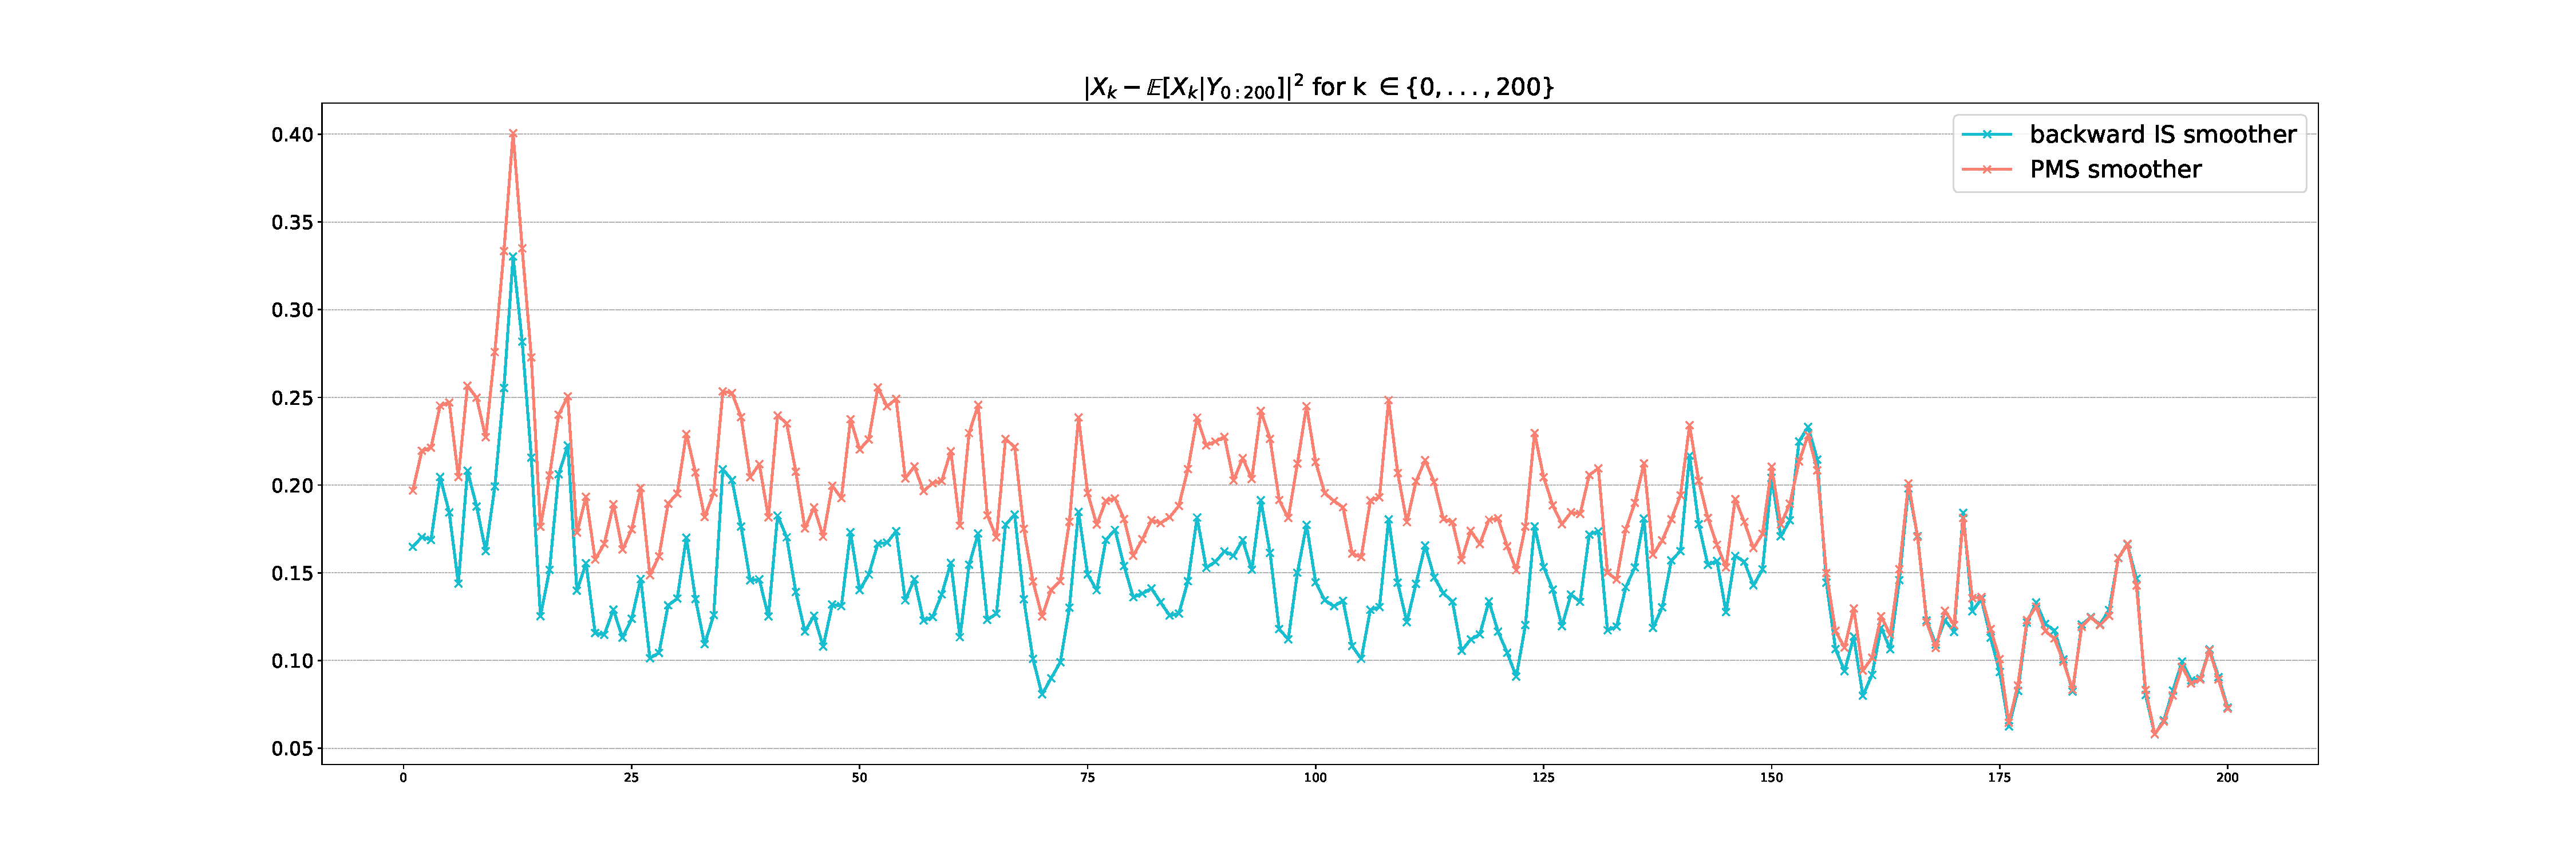
\includegraphics[scale = .3]{RNN_dim64_mse_all_Xk.pdf}
    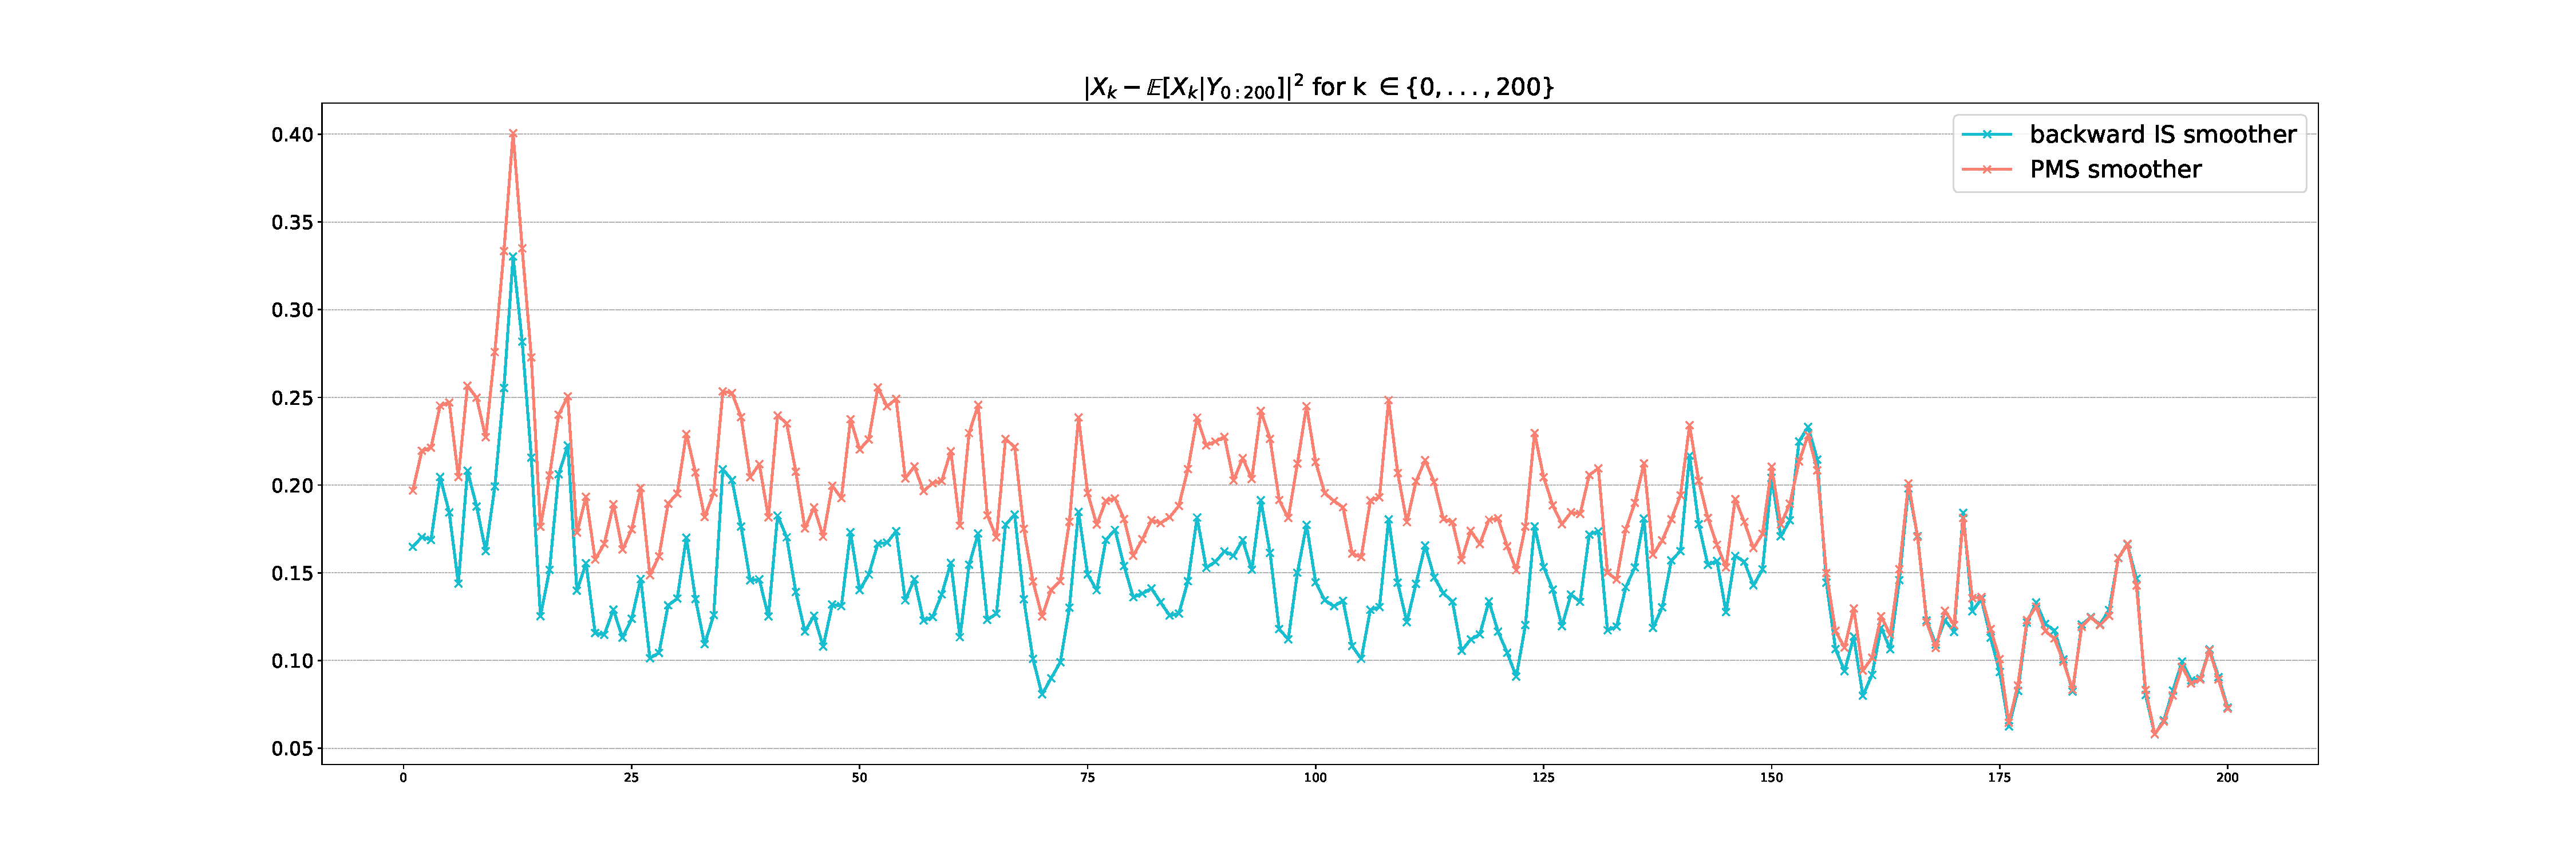
\includegraphics[width=\textwidth, trim = 1cm 1cm 1cm 1cm, clip]{RNN_dim64_mse_all_Xk.pdf}
\end{center}
    \caption{Plot of the empirical estimate of $\mathbb{E}[\|X_k - \mathbb{\widehat{E}}[X_k|Y_{0:199}]\|^2]$ for $k \in \{0,...,199\}$ for 100 runs of the Backward IS and Poor Man smoothers.}
    \label{fig:RNN:mseperXk}
\end{figure}

\subsection{One dimensional diffusion processes: the Sine model}
\label{sec:simu:SINE}
This section investigates the performance of the proposed algorithm to compute  expectations under the smoothing distributions in a context where  alternatives are available for comparison. Consider the Sine model where $(X_t)_{t\geqslant 0}$ is assumed to be a weak solution to
$$
\rmd X_t = \sin(X_t-\theta)\rmd t + \rmd W_t\eqsp,\quad X_0 = x_0\eqsp.
$$
This simple model has no explicit transition density, however, a General Poisson estimator which satisfies \eqref{eq:AR:bound} can be computed by simulating Brownian bridges, (see \cite{beskos2006exact}). 
Therefore, the backward importance sampling technique proposed in this paper can be compared to the usual acceptance-rejection algorithm described in Section~\ref{sec:smoothing}. 
For this simple comparison, observations are received at evenly spaced times $t_0=0,\ldots, t_{10} = 5$ from the model
\begin{equation}
\label{eq:obs:model:SINE}
Y_k=X_{t_k}+\varepsilon_k,\eqsp 0\leqslant k \leqslant n = 10\eqsp,
\end{equation}
where $(\varepsilon_k)_{0 \leqslant k\leqslant 10}$ are i.i.d. Gaussian random variables with mean $0$ and variance $1$. In this experiment $\theta = \pi/4$. 
The proposal distribution $p_k$ for the particle filtering approximation is chosen as the following approximation of the optimal filter:
\begin{equation}
\label{eq:optimal:filter}
p_{k}(x_{k},x_{k+1})\!\propto\! q^{\mathsf{Eul}}_{k+1}(x_{k},x_{k+1})g_{k+1}(x_{k+1},Y_{k+1})\eqsp,
\end{equation}
where $q^{\mathsf{Eul}}_{k+1}$ is the probability density function of Gaussian distibution with mean $\Delta \sin(x_k-\theta)$ and variance $\Delta$ where $\Delta = 1/2$, i.e. the Euler approximation of the Sine SDE, and $g_k$ is the probability density function of the law of $Y_k$ given $X_{t_k}$ i.e. of a Gaussian random variable with mean $X_{t_k}$ and variance 1. 
As the observation model is linear and Gaussian, the proposal distribution is therefore Gaussian with explicit mean and variance. 

In this first experiment, particles are used to solve the state estimation problem for the first observation i.e. to compute an estimate of $ \pE[ X_{0} | Y_{0:n}]$.
Figure~\ref{fig:sine:timeandbias} displays the computational complexity and the estimation of the posterior mean with the acceptance-rejection algorithm and the proposed backward sampling technique as a function of $\K$. 
In this setting, $N=100$, and each unbiased estimate of $\hat{q}$ is computed using 30 Monte Carlo replicates.

For $\K = 2$ (which is the recommended value for the PaRIS algorithm, see \cite{olsson2017efficient}), our estimate shows a bias, which is no surprise, as it is based on a biased normalized importance sampling step. However, this bias quickly vanishes for $\K \geqslant 10$. 
Interestingly, our method comes with a drastic (a factor 10) reduction of computational time. 
The vanishing of the bias might induce more backward sampling, but this remains much faster than the acceptance rejection method with $\K = 2$.

Then, the same estimation was performed (on the same data set) for $\N$ varying from 50 to 2000.
In this context, $\K$ was set to 2 for the AR method. 
To have an empirical intuition of how $\K$ must vary with $\N$, the importance sampling algorithm is applied with $\K = \N^{0.5}, \N^{0.6}$ and $N / 10$ (as this last value was sufficient in the first experiment to avoid any bias). The results are shown in Figure~\ref{fig:sine:timeandbias:N:vary}. A  small bias might appear for $\N = 2000$ and $\K~=~45\eqsp(\approx 2000^{0.5})$, but no bias is visible for $\N^{0.6}$ and $\N /10$. 
%This suggests an heuristic for choosing $\K$, that would have to be confirmed by theoretical results.
As expected, the gain in time, compared to the state of the art algorithm, remains important (even if it decreases as $\K$ increases). 
It is worth noting that the variance of the computational time is greatly reduced compared to the AR technique.% (due to the acceptance rejection step).

\begin{figure}[h]
\begin{center}
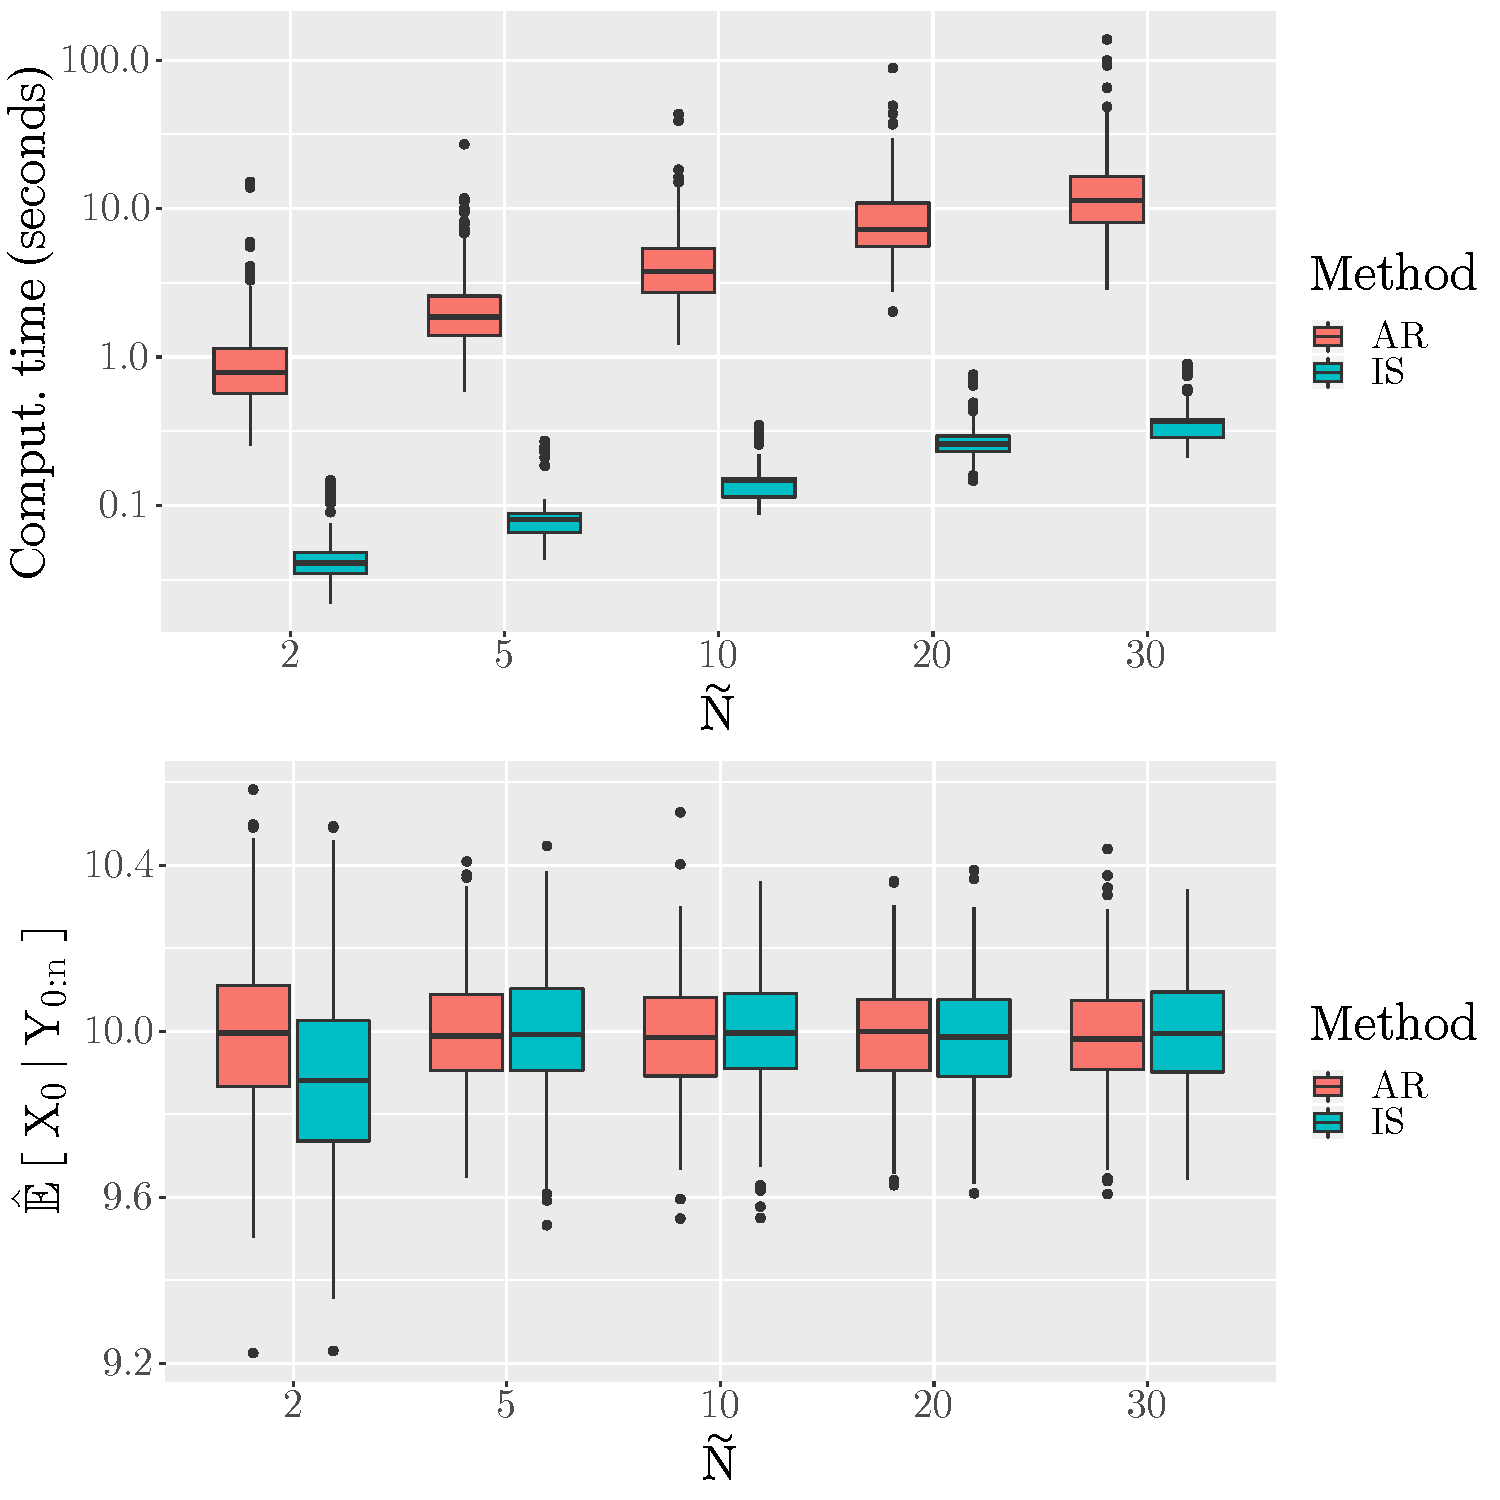
\includegraphics[scale = .4]{comparing_IS_AR_Ntilde_vary.pdf}
\end{center}
\caption{Computational complexity and estimation of a posterior mean as a function of the number of backward samples. Results are shown for the state of the art acceptance-rejection algorithm and the proposed backward importance sampling technique.}
\label{fig:sine:timeandbias}
\end{figure}

\begin{figure}[h]
\begin{center}
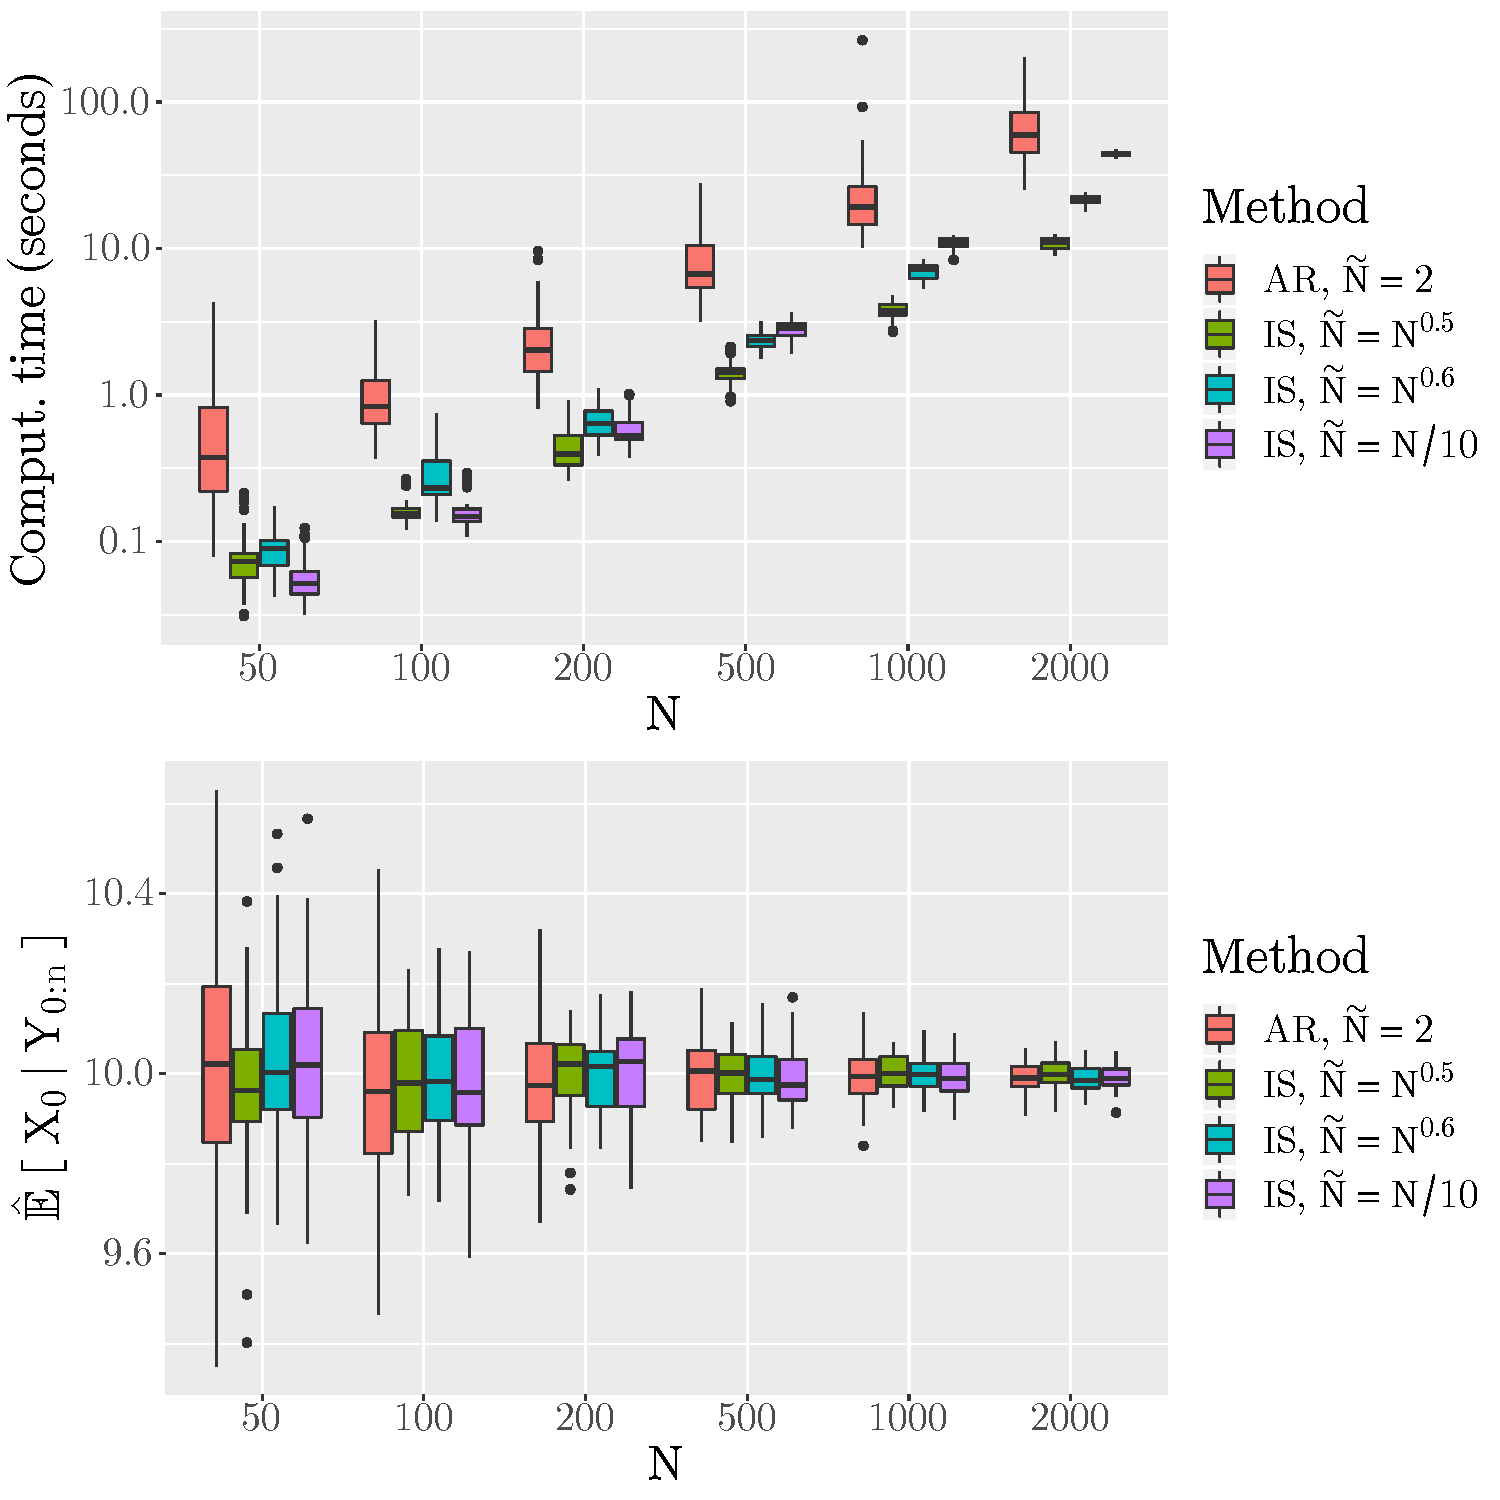
\includegraphics[scale = .4]{comparing_IS_AR_N_vary.pdf}
\end{center}
\caption{Computational complexity and estimation of a posterior mean as a function of the number of particles. Results are shown for the state of the art acceptance-rejection algorithm and the proposed backward  importance sampling technique. The number of backward samples is set to 2 for the AR, and $N/10$ for the IS.}
\label{fig:sine:timeandbias:N:vary}
\end{figure}

\subsection{Multidimensional diffusion processes: Stochastic Lotka-Volterra model}
\label{sec:simu:LV}

This section sets the focus on a stochastic model describing in continuous time the population dynamics in a predator-prey system, as fully discussed in \cite{hening2018persistence}. The bivariate process $(X_t)_{t\geqslant 0}$ of predators and preys abundances is assumed to follow the stochastic  Lotka-Volterra model:
\begin{equation}
\label{eq:LV:SDE}
\rmd X_t = \alpha_\parvec(X_t) \rmd t + \begin{pmatrix}X_1(t) & 0 \\ 0 & X_2(t)\end{pmatrix} \Gamma \rmd \W_t\eqsp,\
\end{equation}
where $\W_t$ is a vector of independent standard Wiener processes, $\Gamma$ a $2\times 2$ matrix, and for $x = (x_1, x_2)^T:$
\[
\alpha_\parvec(x) = \begin{pmatrix} x_1( a_{10} - a_{11}x_1 - a_{12}x_2)\\  x_2(-a_{20} + a_{21}x_1 - a_{22}x_2) \end{pmatrix}\eqsp .
\]
In this context, the unknow parameter to be estimated is $\parvec = ( a_{10}, a_{11}, a_{12}, a_{20}, a_{21}, a_{22}, \Gamma)$. The observation model follows a widespread framework in ecology where the abundance of preys and predators are observed through some abundance index at discrete times $t_0, \dots, t_n$:
\begin{equation}
Y_{t_k} = \begin{pmatrix} \text{c}_1X_1(t_k)\mathrm{e}^{\epsilon^{(1)}_{t_k}} \\ \text{c}_2X_2(t_k)\mathrm{e}^{\epsilon^{(2)}_{t_k}}\end{pmatrix}\eqsp, \label{eq:LV:obs:model}
\end{equation}
where $\text{c} = (\text{c}_1, \text{c}_2)^T$ is known (the observed fraction of the population) and $\lbrace \epsilon_{t_k} =(\epsilon^{(1)}_{t_k}, \epsilon^{(2)}_{t_k})\rbrace_{1\leqslant k\leqslant n}$ are i.i.d. random variables distributed as a $\mathcal{N}_2(-\text{diag}\ \Sigma/2, \Sigma)$ where $\Sigma$ is an unknown 2 $\times$ 2 covariance matrix. It is straightforward to show that for a generic $\parvec$, in the SDE defined by \eqref{eq:LV:SDE}, the drift function cannot be written (even after the Lamperti transform) as the gradient of a potential. 
Therefore, the General Poisson estimator cannot be used as an unbiased estimator of the transition density, and the method proposed in this paper is the only solution to obtain a consistent estimate of  the target expectations. The proposal distribution for the particle filter is again a trade off between model dynamics and the observation model (full details are given in the appendix). The simulated set of particles is used to obtain estimates of the true abundances given the observations, both on synthetic and real data.

\subsubsection*{Synthetic data}

In a first approach,  simulated data are obtained from the model given by \eqref{eq:LV:SDE} and \eqref{eq:LV:obs:model} for a known set of parameters. Chosen values of $\theta$, $\Sigma$, $\text{c}_1$ and $\text{c}_2$ for the experiment are given in the appendix. 
The model is used to simulate abundances indexes $Y_0,\dots Y_{300}$ at times $t_0 = 0,\dots, t_{300} = 3$. 
The associated time series (after a division by $\text{c}$) is shown in Figure \ref{fig:LV:tracking} (left panel). In this experiment, the goal is to obtain an estimate of the actual predator-prey abundances given all the observed abundances indexes $Y_{0:n}$. 
Our estimate is given by the set of conditional expectations $\lbrace\pE[ X_k \vert Y_{0:n}]\rbrace_{k = 0,\dots, n}$, approximated using our backward importance sampling PaRIS smoother, which is run using the true parameters. 
Figure \ref{fig:LV:tracking} shows the estimated abundance trajectory over time. 
The proposed algorithm manages to estimate efficiently the actual abundance from noisy data and a model with an intractable transition density.

\begin{figure}
\begin{center}
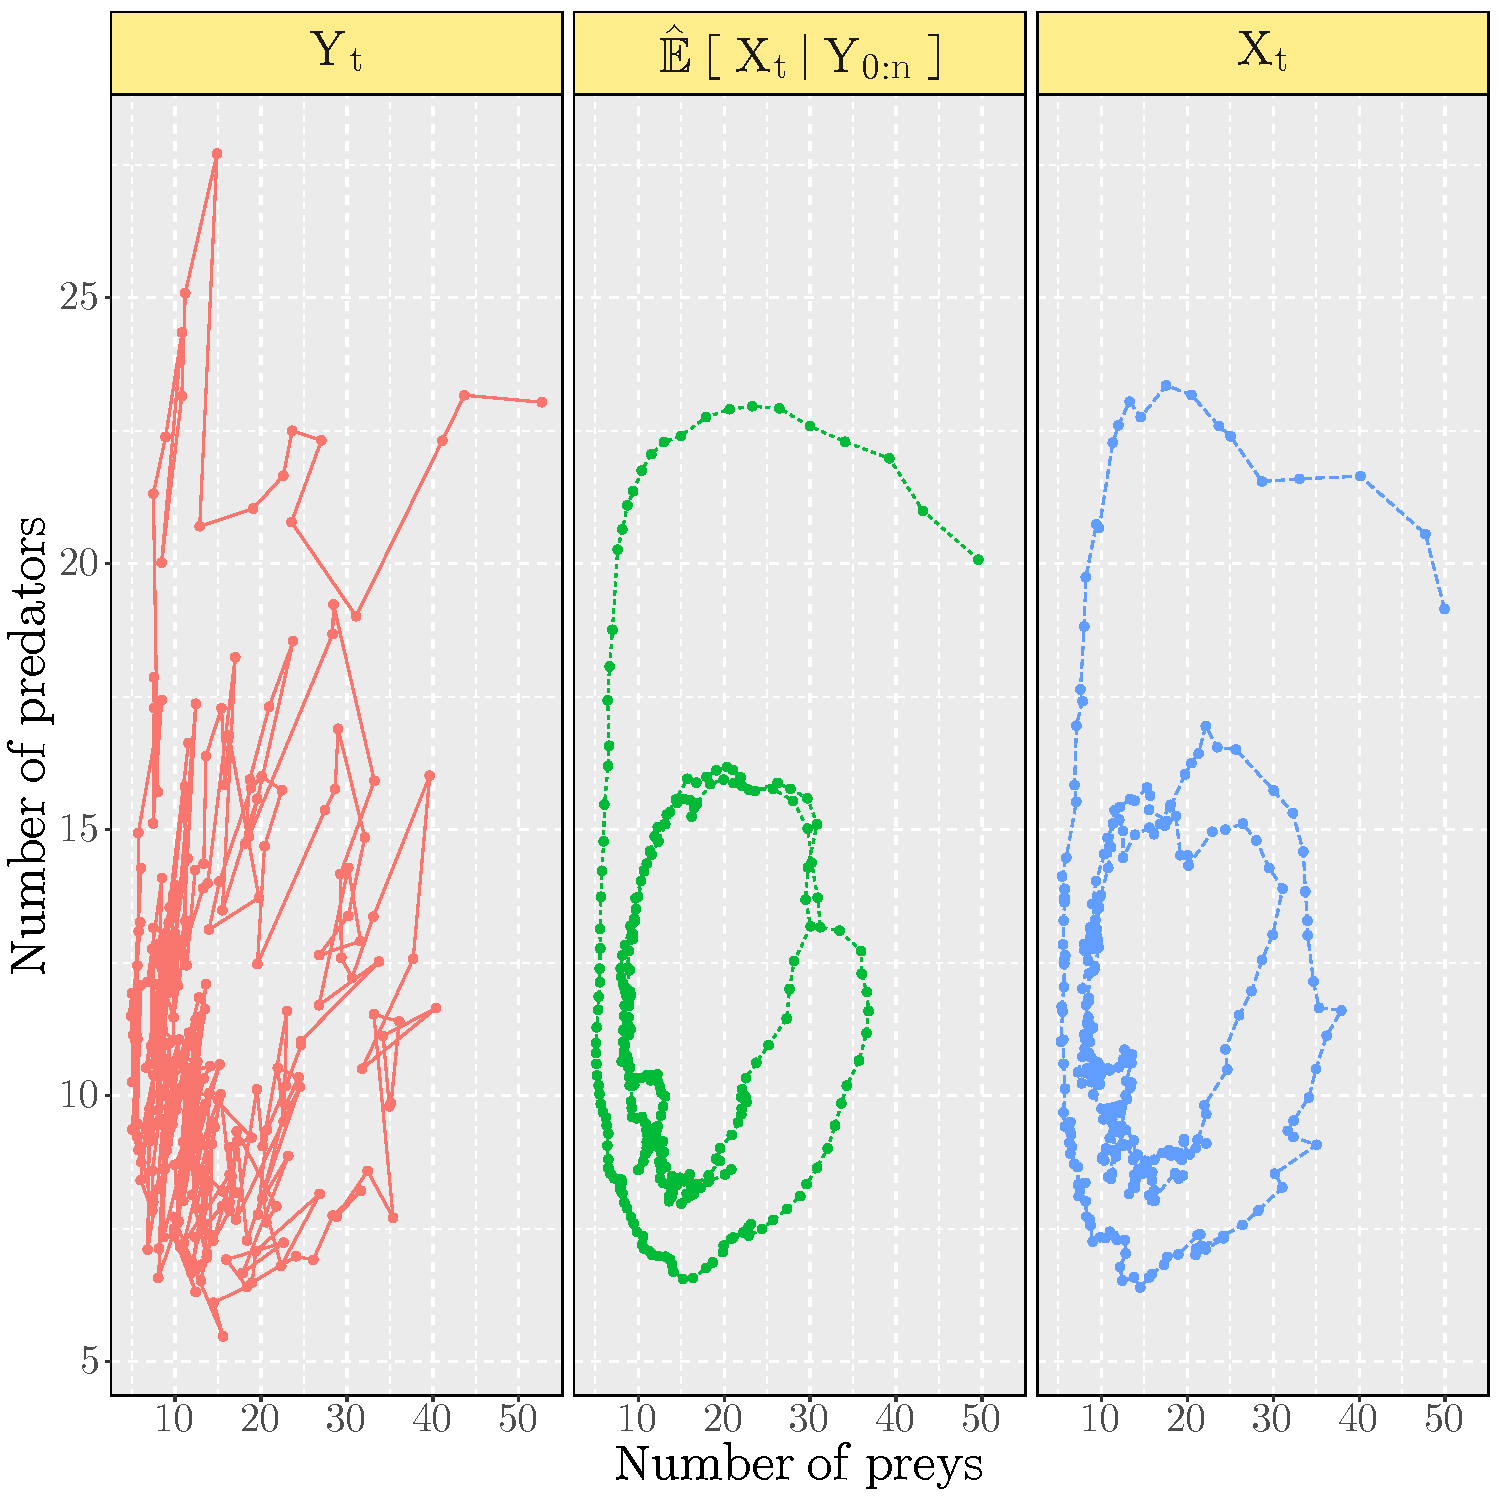
\includegraphics[scale = .4]{smoothed_tracking_LV.pdf}
\end{center}
\caption{\label{fig:LV:tracking} Estimated predator-prey abundances (center) in a stochastic Lotka Volterra model using our backward sampling estimate on simulated abundance indexes (left). Right panel shows the ground truth.}
\end{figure}

\subsubsection*{Hares and lynx data}

In this section, the model defined by equations \eqref{eq:LV:SDE} and \eqref{eq:LV:obs:model} is applied to the Hudson Bay company data, giving the number of hares and lynx trapped in Canada during the first 20 years of the 20th century (available in \cite{odum1971fundamentals}). As parameters are unknown in this case, maximum likelihood inference is performed using an EM \cite{dempster1977maximum} algorithm to obtain an estimate $\hat{\theta}$.
As explained in the introduction, it is then required to estimate iteratively, from an initial guess $\theta_0$, the conditional expectation given in equation \eqref{eq:EM:E:step}.
This E step is performed using the particle smoother introduced in this paper.
At each iteration, the estimator $\theta_k$ is updated by finding a parameter $\theta_{k+1}$ for which $\hat Q(\theta_{k+1},\theta_k) >  \hat Q(\theta_k,\theta_k)$, with  a gradient free evolution strategy \cite{hansen2006cma}. The last estimate $\hat{\theta}$ obtained with this EM algorithm  is used to  estimate the actual abundances in the model (similarly to the synthetic data case). Figure \ref{fig:LV:hares:lynx} shows  estimates of $\pE_{\hat{\theta}}\left[ X_k \vert Y_{0:n}\right]$ obtained with 30 independent runs of our algorithm. 
The particle smoother is implemented using $N = 200$ particles and $\tilde{N}=20$. 
The replicates show that the variance of our estimator (for a given set of observations) is much smaller than the one of the {\em poor man smoother}. This algorithm approximates the smoothing distributions at time $n$ by the weighted samples  where the particle trajectories $\epart{0:n}{\ell}$, $1\leqslant \ell \leqslant N$,  are obtained using the ancestral line of each last sample. The variance of the estimates based on this ancestor tree is doomed to failure due to the degeneracy caused by the successive resampling steps.

\section{Online recursive maximum likelihood}

%\subsection{Particle based online estimation}
%\label{sec:tangent:filter}

This section focuses on the context of online recursive maximum likelihood, i.e., where new observations are used only once to update the estimator of the unknown parameter $\parvec$.
%We first fully describe the algorithm and its particle based implementation. At the end of the section, we give the main arguments behind the method.
Following \cite{legland1997recursive}, the idea is the build a sequence $\left\lbrace\parvec_k\right\rbrace_{k\geq 0}$ as follows. First, set the initial value of the parameter estimate: $\parvec_0$. The, for each new observation $Y_{k},~k\geqslant 1$, define
$$
\theta_{k} = \theta_{k-1} + \gamma_k \deriv \logllh{\parvec}(Y_k \mid Y_{1:k - 1}) \eqsp,
$$
where $\logllh{\parvec}(Y_k \mid Y_{1:k - 1})$ is the log likelihood for the new observation given all the past, and $\left\lbrace\gamma_k\right\rbrace_{k\geqslant}$ are positive step sizes such that $\sum_{k \geqslant 1}\gamma_k = \infty$ and $\sum_{k \geqslant 1}\gamma_k^2 < \infty$. The practicalt implementation of such an update relies on the following identity:
\begin{equation}
\deriv \logllh{\parvec}(Y_k \mid Y_{1:k - 1})  
=  \frac{\pred{k;\parvec}[\deriv \md{k;\parvec}] + \filtderiv{k;\parvec}[\md{k;\parvec}]}{\pred{k;\parvec}[\md{k;\parvec}]}\eqsp,
\label{eq:online:gradient}
\end{equation}
where $\pred{k;\parvec} = \phi_{k;\parvec \mid k - 1}$ is the predictive distribution  and 
$$\filtderiv{k;\parvec}[\md{k;\parvec}] = \post{0:k;\parvec \mid k - 1} [\af{0:k;\parvec} \md{k;\parvec}] - \pred{k;\parvec}[\md{k;\parvec}] \times \post{0:k;\parvec \mid k - 1 }[\af{0:k}]\eqsp,$$
with
\begin{equation}
\label{eq:complete:gradient:log}
\af{0:k}(x_{0:k}) =  \sum_{j = 0}^{k - 1} \deriv\log \qg{j, \parvec}(x_j,x_{j+1})\eqsp.
\end{equation}
%$$\filtderiv{k;\parvec}[\md{k;\parvec}] = \int \md{k;\parvec}(x_k) \deriv \pred{k;\parvec}(x_k) \rmd x_k,$$
The signed measure $\filtderiv{k;\parvec}$ is known as the \textit{tangent filter}, see \cite[Chapter~10]{cappe2005inference}, \cite{delmoral2015uniform} or \cite{olsson2020particle}. 
%In order to build a particle-based approximation of $\eqref{eq:online:gradient}$, we can remark that
%$$\filtderiv{k;\parvec}[\md{k;\parvec}] = \post{0:k;\parvec \mid k - 1} [\af{0:k;\parvec} \md{k;\parvec}] - \pred{k;\parvec}[\md{k;\parvec}] \times \post{0:k;\parvec \mid k - 1 }[\af{0:k}]\eqsp,$$
%where 
%\begin{equation}
%\label{eq:complete:gradient:log}
%\af{0:k}(x_{0:k}) =  \sum_{j = 0}^{k - 1} \deriv\log \qg{j, \parvec}(x_j,x_{j+1})\eqsp.
%\end{equation}
Using the tower property  and the backward decomposition \eqref{eq:property:backward} yields
\begin{equation} 
\label{eq:tangent:identity}
\filtderiv{k;\parvec}[\md{k;\parvec}] = \pred{k;\parvec}\left[\left(\tstat{k} [\af{0:k}] - \pred{k;\parvec}[\tstat{k}[\af{0:k}]]\right) \md{k;\parvec}\right]\eqsp.
\end{equation}
Therefore, a particle filter, can be used to compute the following seuqential Monte Carlo approximation:
$$
\pred{k}^N[\md{k;\parvec}] = \frac{1}{N}\sum_{\ell = 1}^N \md{k;\parvec}(\epart{n}{\ell})\eqsp,\eqsp \pred{k}^N[\deriv \md{k;\parvec}] = \frac{1}{N}\sum_{\ell = 1}^N \deriv \md{k;\parvec}(\epart{k}{\ell})\eqsp.
$$
In addition, the thangent filter can be approximated using a backward sampling procedure, based on the backward statistic associated with  the functional \eqref{eq:complete:gradient:log}:
\begin{equation} 
\label{eq:tangent:identity:part:linear}
\eta_{k;\parvec}^{N}[\md{k;\parvec}] = \frac{1}{\N}\sum_{\ell=1}^\N\tau_\ell^k \md{k;\parvec}
(\epart{\ell}{k}) - \left(\frac{1}{\N}\sum_{\ell=1}^\N\tau_\ell^n\right)\left(\frac{1}{\N}\sum_{\ell=1}^\N \md{k;\parvec}(\epart{\ell}{k})\right)\eqsp.
\end{equation}
Plugging these estimates in equation \eqref{eq:online:gradient} allows to perform the online recursive algorithm. It is worth noting that, in the context of this paper where $\qg{k}$ cannot be evaluated pointwise, one cannot expect to know the functional \eqref{eq:complete:gradient:log}, which involves the gradient of this quantity. 
In section \ref{sec:xp:tangent:filter}, we illustrate that we can plug-in an estimate of this functionnal instead. The rationale motivating this algorithm relies on the following expression of the normalized loglikelihood:
$$
\frac{1}{n} \deriv \logllh{\parvec}(Y_{1:n}) = \frac{1}{n} \sum_{k = 1}^n \deriv \logllh{\parvec}\left(Y_k \mid Y_{1:k - 1}\right)\eqsp.$$
Moreover, under strong mixing assumptions, for all  $\parvec \in \parvec$, the extended process $\{ (X_n, Y_n, \pred{n}, \filtderiv{n}) \}_{n \geqslant 0}$ is an ergodic Markov chain and for all $\parvec \in \parvec$, the normalized score $\deriv \logllh{\parvec}(Y_{1:n})/n$  converges almost surely to a limiting quantity $\lambda(\parvec, \parvec_{\star})$ such that, under identifiability constraints, $\lambda(\parvec_{\star}, \parvec_{\star}) = 0$. 
A gradient ascent algorithm cannot be designed as the limiting function $\parvec \mapsto \lambda(\parvec, \parvec_{\star})$ is not available explicitly. 
However, solving the equation $\lambda(\parvec_{\star}, \parvec_{\star}) = 0$ may be cast into the framework of \emph{stochastic approximation} to produce parameter estimates using the \emph{Robbins-Monro algorithm}
\begin{equation}
\label{eq:par:update}
\parvec_{k} = \parvec_{k - 1} + \gamma_{k} \zeta_{k}\eqsp, \quad n\geqslant 0\eqsp, 
\end{equation}
where $\zeta_{k}$ is a noisy observation of $\lambda(\parvec_{k - 1}, \parvec_{\star})$, equal to \eqref{eq:online:gradient}.  
In the case of a finite state space $\set{X}$ the algorithm was studied in~\cite{legland1997recursive}, which also provides assumptions under which the sequence $\{\parvec_{n}\}_{n\geqslant 0}$ converges towards the parameter $\parvec_{\star}$ (see also \cite{tadic2010analyticity} for refinements). 
%
%
%As noted for instance in \cite[Section~2]{delmoral2015uniform} and \cite{olsson2017efficient}, for all $\parvec\in\parspace$ and all bounded and measurable function $f_{0:n}$ on $(\Xset)^{n+1}$,
%\[
%\deriv \post{0:n;\parvec \mid n - 1}[f_{0:n}]  = \post{0:n;\parvec \mid n - 1} [\af{n} f_{0:n}] - \post{0:n;\parvec \mid n - 1} [f_{0:n}] \times \post{0:n;\parvec \mid n - 1 }[\af{n}]\eqsp,
%\]
%where
%\begin{equation*}
%\af{n}(x_{0:n}) = \sum_{k=0}^{n-1}\addf{k;\parvec}(x_{k},x_{k+1})\eqsp,
%\end{equation*}
%with, for all $0\leqslant k \leqslant n-1$,
%\[
%\addf{k;\parvec}(x_{k},x_{k+1}) = \nabla_{\parvec}\log \md{k+1;\parvec}(x_{k+1},Y_{k+1}) + \nabla_{\parvec}\log \hd{k;\parvec}(x_k,x_{k+1})\eqsp.
%\]
%Considering an objective function $f_{n}$ defined on $\Xset$ which depends on the last state $x_n$ only, the tangent filter $\filtderiv{n}$ is defined as the following signed measure: 
%$$
%\filtderiv{n;\parvec}[f_n] \eqdef \deriv \pred{n;\parvec}[f_n] = \post{0:n;\parvec \mid n - 1} [\af{n;\parvec} f_{n}] - \pred{n;\parvec}[f_{n}] \times \post{0:n;\parvec \mid n - 1 }[\af{n}]\eqsp, 
%$$
%where $\pred{n}=\post{n:n\mid n - 1}$ is the predictive measure. 
%The particle based estimator of $\pred{n}[f]$ is given by:
%$$\pred{n}^N[f] = \frac{1}{N}\sum_{\ell = 1}^N f(\epart{n}{\ell})\eqsp.$$
%Using the tower property  and the backward decomposition \eqref{eq:property:backward}:
%\begin{equation} 
%\label{eq:tangent:identity}
%\filtderiv{n;\parvec}[f_n] = \pred{n;\parvec}[(\tstat{n} [\af{n}] - \pred{n;\parvec}[\tstat{n}[\af{n}]]) f_n]\eqsp.
%\end{equation}
%Therefore, the tangent filter \eqref{eq:tangent:identity} can be approximated on-the-fly using the statistics $(\tau_i^n)_{i=1}^{\N}$ and the weighted particles $\{(\epart{n}{i}, \ewght{n}{i})\}_{i=1}^{\N}$:
%%\begin{equation} 
%%\label{eq:tangent:identity:part}
%%\filtderiv{n;\parvec}^{N,\textrm{FFBS}}[f_n] = \frac{1}{\N}\sum_{i=1}^\N\tstattil{i}{n}f_n(\epart{i}{n}) - \left(\frac{1}{\N}\sum_{i=1}^\N\tstattil{i}{n}\right)\left(\frac{1}{\N}\sum_{i=1}^\N f_n(\epart{i}{n})\right)\eqsp.
%%\end{equation}
%%In cases where $\qg{k}$, $0\leqslant k \leqslant n-1$, is unknown and replaced by an unbiased estimate, the associated pseudo marginal particle-based approximation of the tangent filter is given by:
%\begin{equation} 
%\label{eq:tangent:identity:part:linear}
%\eta_{n;\parvec}^{N}[f_n] = \frac{1}{\N}\sum_{i=1}^\N\tau_i^n f_n(\epart{i}{n}) - \left(\frac{1}{\N}\sum_{i=1}^\N\tau_i^n\right)\left(\frac{1}{\N}\sum_{i=1}^\N f_n(\epart{i}{n})\right)\eqsp.
%\end{equation}
%%\textcolor{red}{To be adapted if $g_{k}$ depends on both $x_k$ and $x_{k+1}$. As it is more an application of the results displayed in the previous section, I do think that this should be written as it is, with $g_{k}$ depending only on $x_k$. This is the version used in the experiments and this is the one given in the paper with Westerborn...}.
%Given a set of observations $Y_{1:n}$, maximum likelihood estimation amounts at obtaining a parameter $\hat\parvec_{n} \in \parspace$ such that $\hat\parvec_{n} = \arg\max_{\parvec \in \parspace} \logllh{\parvec;n}(Y_{1:n})$, where $\logllh{\parvec;n}(Y_{1:n}) = \log \llh{\parvec;n}(Y_{1:n})$ is the logarithm of the likelihood. There are many different approaches to compute an estimator of $\hat\parvec_{n}$, see for instance~\cite[Chapter 10]{cappe2005inference}. Following \cite{douc2001asymptotics}, under strong mixing assumptions, for all  $\parvec \in \parvec$, the extended process $\{ (X_n, Y_n, \pred{n}, \filtderiv{n}) \}_{n \geqslant 0}$ is an ergodic Markov chain and for all $\parvec \in \parvec$, the normalized score $\deriv \logllh{\parvec}(Y_{1:n})/n$ of the observations may be shown to converge where:
%\[
%\frac{1}{n} \deriv \logllh{\parvec}(Y_{1:n}) = \frac{1}{n} \sum_{k = 1}^n \deriv \logllh{\parvec}(Y_k \mid Y_{1:k - 1})  
%=  \frac{1}{n} \sum_{k = 0}^n \frac{\pred{k;\parvec}[\deriv \md{k;\parvec}] + \filtderiv{k;\parvec}[\md{k;\parvec}]}{\pred{k;\parvec}[\md{k;\parvec}]}\eqsp.
%\]
%Assuming that the observations $Y_{1:n}$ are generated by a model driven by a true parameter $\parvec_{\star}$ for all $\parvec\in\parvec$ this normalized score converges almost surely to a limiting quantity $\lambda(\parvec, \parvec_{\star})$ such that, under identifiability constraints, $\lambda(\parvec_{\star}, \parvec_{\star}) = 0$. A gradient ascent algorithm cannot be designed as the limiting function $\parvec \mapsto \lambda(\parvec, \parvec_{\star})$ is not available explicitly. Solving the equation $\lambda(\parvec_{\star}, \parvec_{\star}) = 0$ may be cast into the framework of \emph{stochastic approximation} to produce parameter estimates using the \emph{Robbins-Monro algorithm}
%\begin{equation}
%\label{eq:par:update}
%\parvec_{n+1} = \parvec_n + \gamma_{n+1} \zeta_{n+1}\eqsp, \quad n\geqslant 0\eqsp, 
%\end{equation}
%where $\zeta_{n+1}$ is a noisy observation of $\lambda(\parvec_n, \parvec_{\star})$. Obtaining such an observation is not possible in practice and following \cite{olsson2017efficient} this noisy observation is approximated by 
%\begin{equation} 
%\label{eq:def:zeta}
%\zeta_{n + 1} \eqdef \frac{\zeta^{1}_{n+1} + \zeta^{2}_{n+1}}{\zeta^{3}_{n+1}}\eqsp,
%\end{equation}
%where
%\begin{equation} 
%\label{eq:zeta:terms}
%\zeta^{1}_{n+1} \eqdef \pred{n+1;\parvec_n} \left[ (\deriv \md{n+1;\parvec})_{|{\parvec = \parvec_n}} \right]\eqsp,  \quad \zeta^{2}_{n+1} \eqdef \filtderiv{n+1;\parvec_n}[\md{n + 1;\parvec_n}]\quad \mbox{and} \quad\zeta^{3}_{n+1} \eqdef \pred{n+1;\parvec_n}[\md{n + 1;\parvec_n}]\eqsp.
%\end{equation}
%In \eqref{eq:zeta:terms}, the measures $\pred{n+1;\parvec_n}$ and $\filtderiv{n+1;\parvec_n}$ depend on \emph{all} the past parameter values. In the case of a finite state space $\set{X}$ the algorithm was studied in~\cite{legland1997recursive}, which also provides assumptions under which the sequence $\{\parvec_{n}\}_{n\geqslant 0}$ converges towards the parameter $\parvec_{\star}$ (see also \cite{tadic2010analyticity} for refinements). In more general cases, these measures may be estimated online using the pseudo marginal smoother presented in this paper.
%%The PaRIS based approximations of the tangent filter and the recursive maximum likelihood estimator are given in Appendix~\ref{sec:alg}.
%
%
%


\subsection{Experiments: online estimation in the SINE model}
\label{sec:xp:tangent:filter}
Online recursive maximum likelihood using pseudo marginal SMC is illustrated for the SINE model of section \ref{sec:simu:SINE}. 
As mentionned, a GPE estimator of the transition density can be computed. 
Following the idea of this computation, one can actually obtain an unbiased estimated of the gradient of the log-transition density, and thus compute and unbiased estimate of the key quantity given in \eqref{eq:complete:gradient:log}. 
To the best of our knowledge, this estimator is new, and given in appendix \ref{sec:filter:SDE}.

A simulated data set is displayed in Figure~\ref{fig:data}, where $\parvec_* = \pi/4$. The solution to the SINE SDE is sampled at times $(t_k)_{0\leqslant k\leqslant n}$  using the Exact algorithm of \cite{beskos2006retrospective}. 
For all  $0\leqslant k \leqslant n-1$,  $\widehat{q}_{k,\parvec}$ and the GPE unbiased estimator of $\nabla_{\parvec}q_{k,\parvec}(x,y)$ are estimated using $M = 30$ independent Monte Carlo replications of the general Poisson estimator. 
The estimations of $\parvec_*$ are given for $50$ independent runs started at random locations $\theta_0$ with $\N = 100$ particles and $\K = 2$ backward samples. Following \cite{gloaguen2018online}, the proposal distribution of the particle filter is obtained using an approximation of the fully adapted particle filter where $\hd{k,\parvec}$ is replaced by the its Euler scheme approximation.


{\em Sensitivity to the starting point $\hat{\parvec}_0$.}
The inference procedure was performed on the same data set from 50 different starting points uniformly chosen in $(0,2\pi)$. The gradient step size $\gamma_k$ of equation \eqref{eq:par:update} was chosen constant (and equal to 0.5) for the first 300 time steps, and then decreasing with a rate proportional to $k^{-0.6}$. Results are given Figure~\ref{fig:1obs:50start}. There is no sensitivity to the starting point of the algorithm, and after a couple of hundred observations, the estimates all concentrate around the true value. As the gradient step size decreases, the estimates stay around the true value following autocorrelated patterns that are common to all trajectories.

{\em Asymptotic normality.}
The inference procedure was performed on 50 different data sets simulated with the same $\theta_*$. The 50 estimates were obtained starting from the same starting point (fixed to $\theta_*$, as Figure \ref{fig:1obs:50start} shows no sensitivity to the starting point). Figure \ref{fig:50obs:1start} shows the results for the raw and the averaged estimates. 
 The averaged estimates $(\widetilde \parvec_k)_{k\geqslant 0}$ consist in averaging the values produced by the estimation procedure after a burning phase of $n_0$ time steps (here $n_0 =300$ time steps). This procedure allows to obtain an estimator whose convergence rate does not depend on the step sizes chosen by the user, see \cite{polyak1992acceleration,kushner1997stochastic}. For all $0 \leqslant k\leqslant n_0$, $\widetilde \parvec_k = \widehat\parvec_k $ and for all $k>n_0$,
\[
\widetilde \parvec_k = \frac{1}{k-n_0}\sum_{j= n_0+1}^k\widehat\parvec_j\eqsp. 
\]
As expected, the estimated distribution of the final estimates tends to be Gaussian, centered around the true value.
 
{\em Step size influence.} To illustrate the  influence of the gradient step sizes, different settings are considered. In each scenario, the sequence $(\gamma_k)_{k\geqslant 0}$ is given by
\begin{equation*}
\gamma_k = \gamma_0 \1_{\left\lbrace k \leq n_0 \right\rbrace} + \frac{\gamma_0}{(k - n_0)^{\kappa}}\1_{\left\lbrace k > n_0 \right\rbrace}\eqsp,
\end{equation*}
where $\gamma_0 = 0.5$. In this experiment $\kappa\in\{0.5,0.6,0.7,0.8,0.9,1\}$.
The results are shown in Figure~\ref{fig:1obs:1start:6Grads}. 
As expected, the raw estimator shows different rates of convergence depending on $\kappa$, whereas the averaged estimator has the same behavior in all cases. 

\begin{figure}
\centering
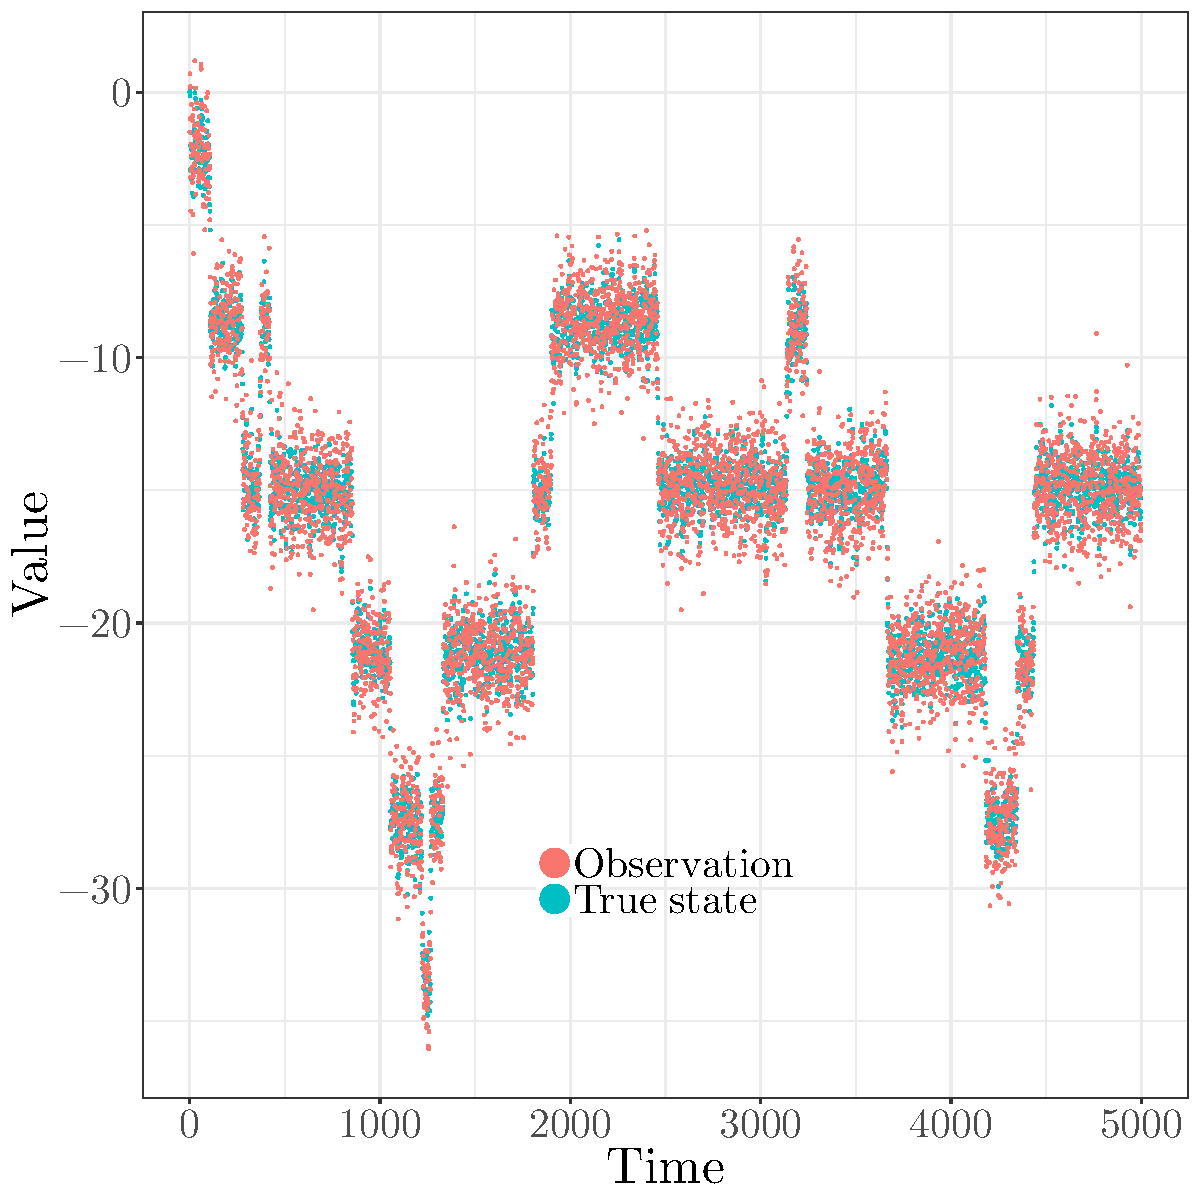
\includegraphics[width = 0.7\textwidth]{SINE_data.pdf}
\caption{\label{fig:data} Data set simulated according to the SINE process, observed with noise at discrete time steps.}
\end{figure}
\begin{figure}
\centering
\begin{tabular}{cc}
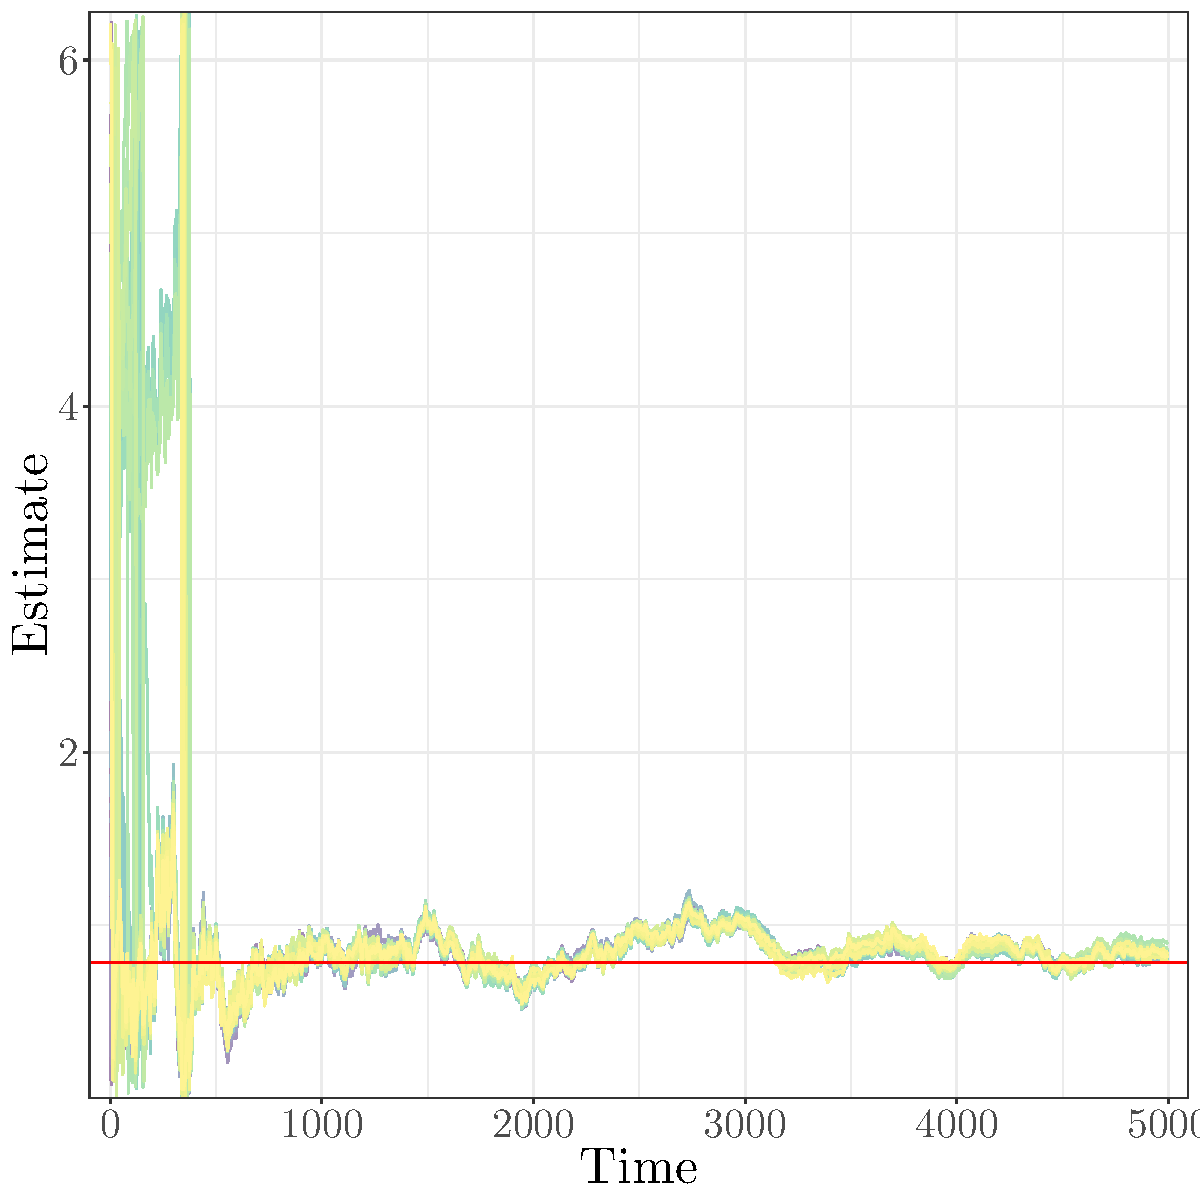
\includegraphics[width = 0.4\textwidth]{oneObs_severalStarts.pdf}&
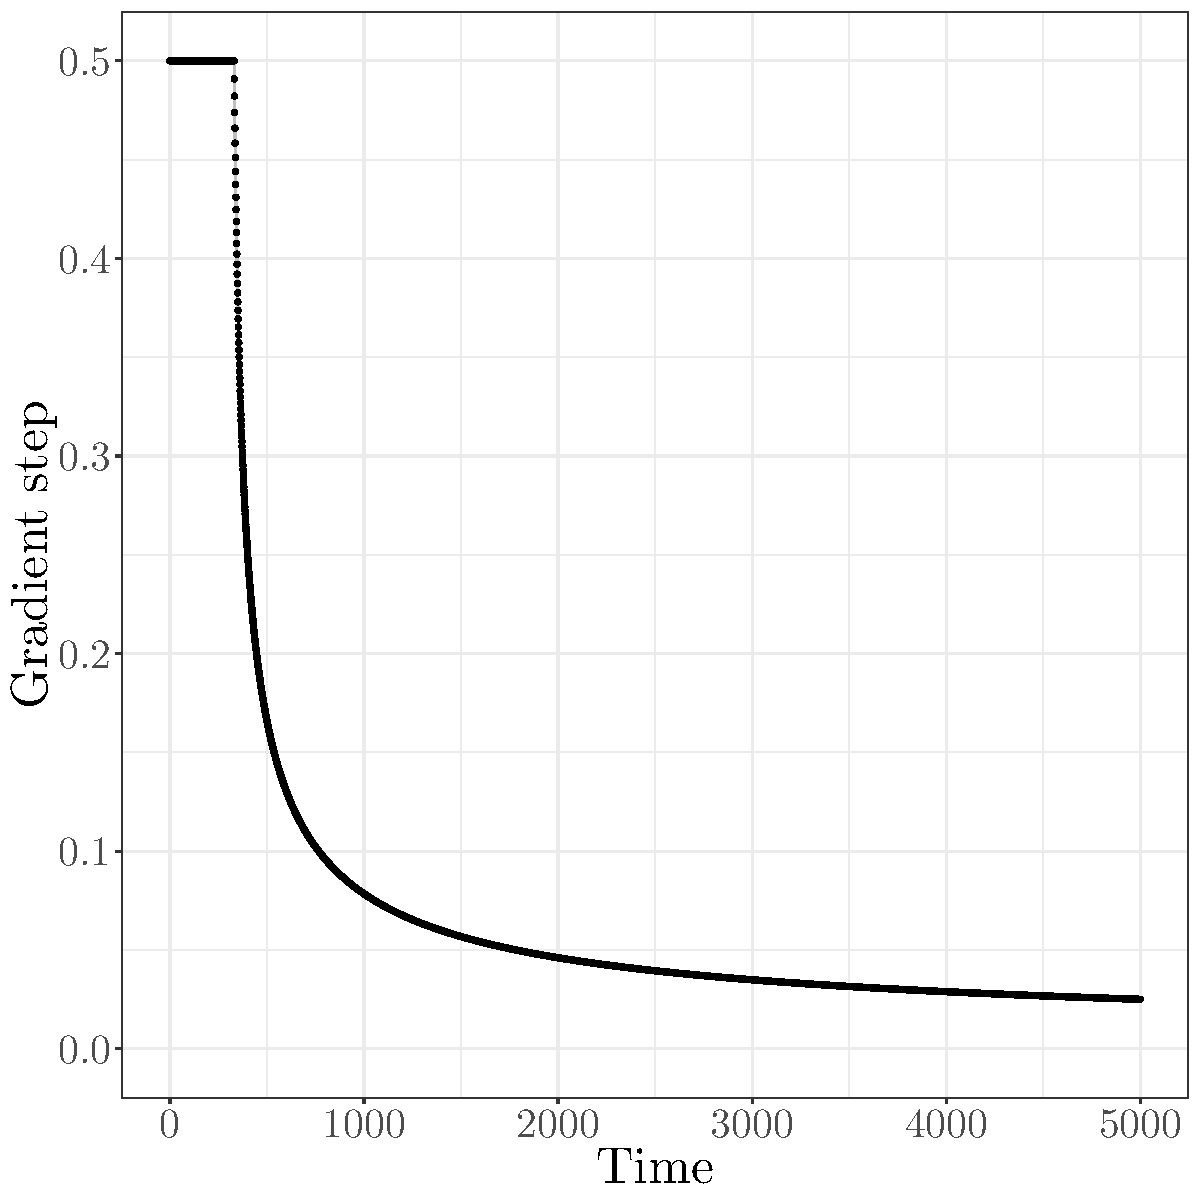
\includegraphics[width = 0.4\textwidth]{gradient_steps.pdf}
\end{tabular} 
\caption{\label{fig:1obs:50start}(\textit{Left}) online estimation of $\parvec$ for the data set presented in Figure~\ref{fig:data}. The algorithm is performed from 50 starting points. (\textit{Right}) The gradient step sizes (defined in equation \eqref{eq:par:update}).}
\end{figure}
\begin{figure}
\centering
\begin{tabular}{ccc}
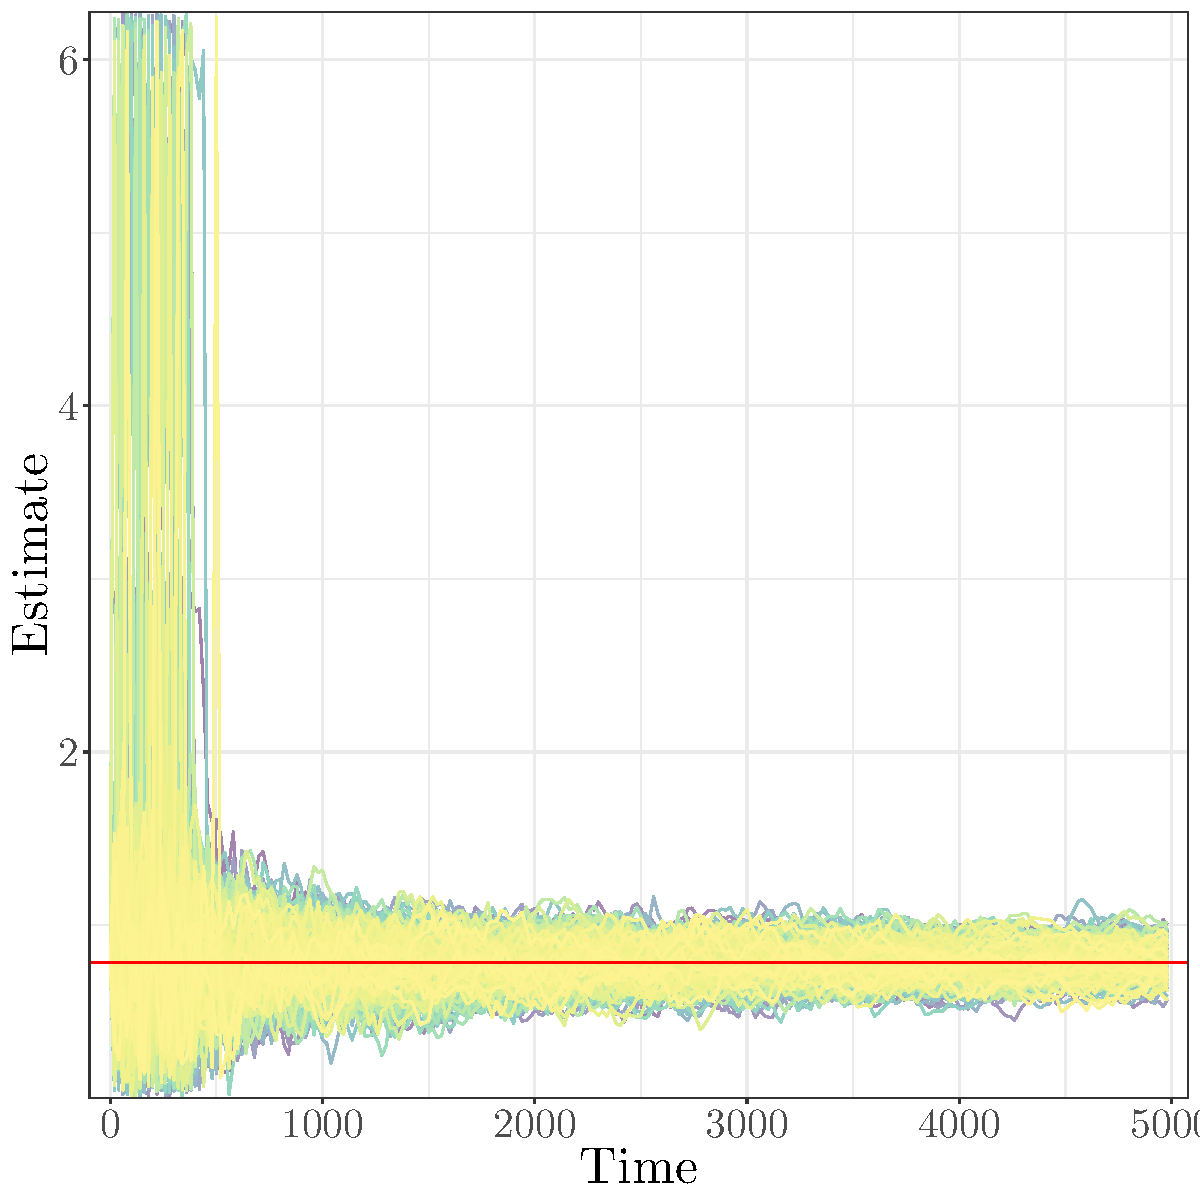
\includegraphics[width = 0.32\textwidth]{severalObs_oneStart.pdf}&
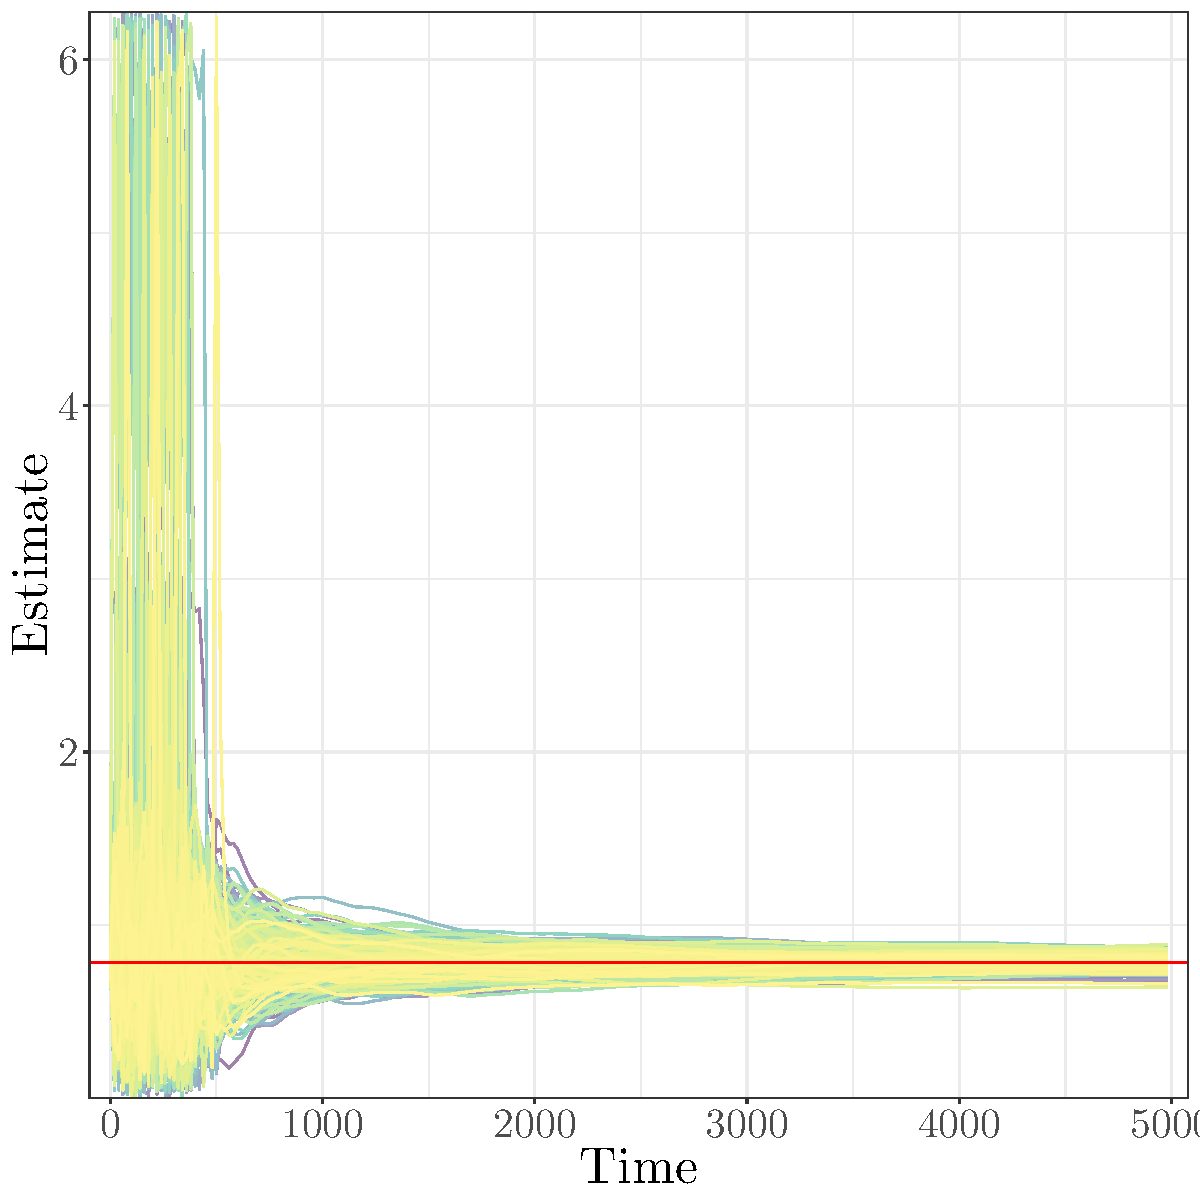
\includegraphics[width = 0.32\textwidth]{severalObs_oneStart_smooth.pdf}&
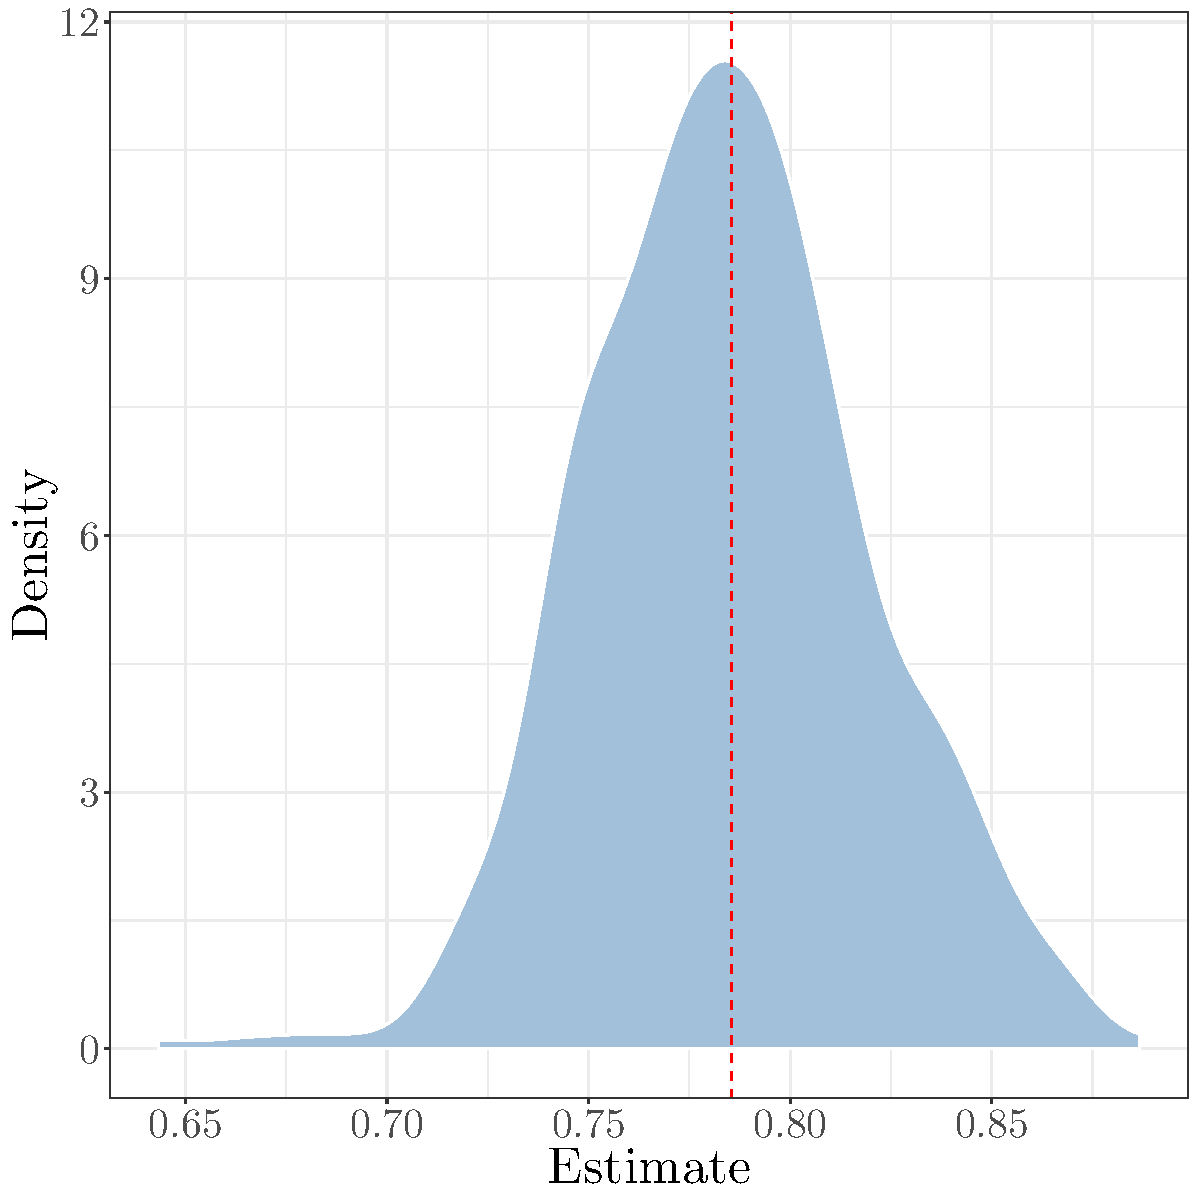
\includegraphics[width = 0.32\textwidth]{severalObs_oneStart_smooth_dens.pdf}
\end{tabular}
\caption{\label{fig:50obs:1start}(\textit{Left}) online estimation of $\parvec$ for 50 different simulated data sets as presented in Figure \ref{fig:data}. The algorithm is performed from 1 starting point with the gradient step size shown in Figure \ref{fig:1obs:50start}. (\textit{Center}) Averaged estimator, where $\hat{\parvec}$ is averaged after a burning phase of 300 time steps. (\textit{Right}) Empirical distribution of $\hat{\parvec}$. The red line is the value of $\parvec^*$.}
\end{figure}

\begin{figure}
\centering
\begin{tabular}{cc}
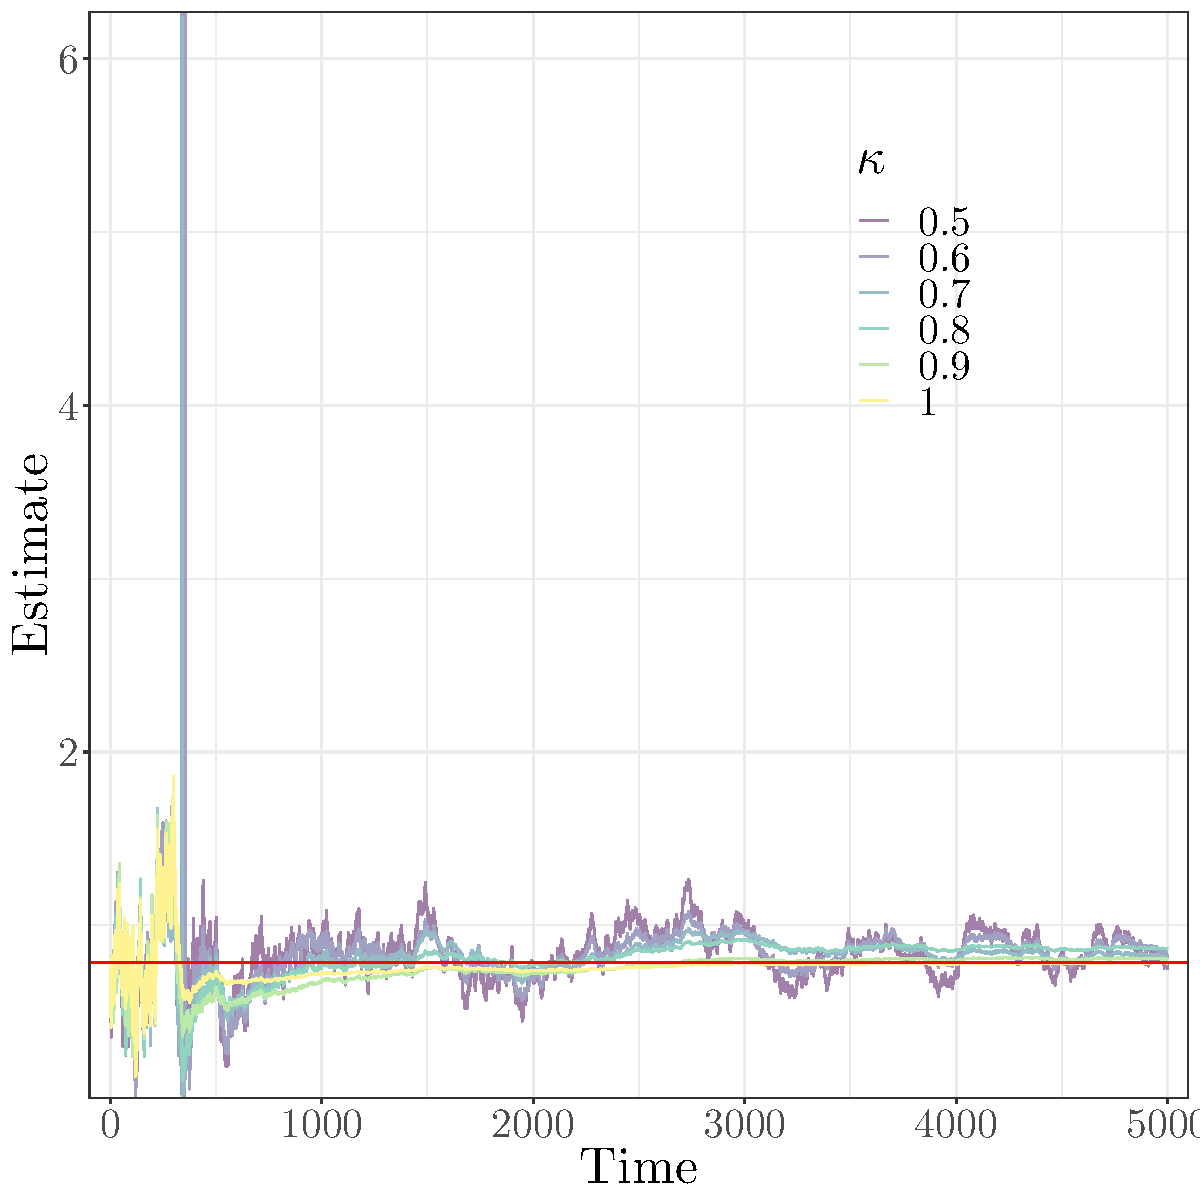
\includegraphics[width = 0.4\textwidth]{oneObs_oneStart_severalGrads.pdf}&
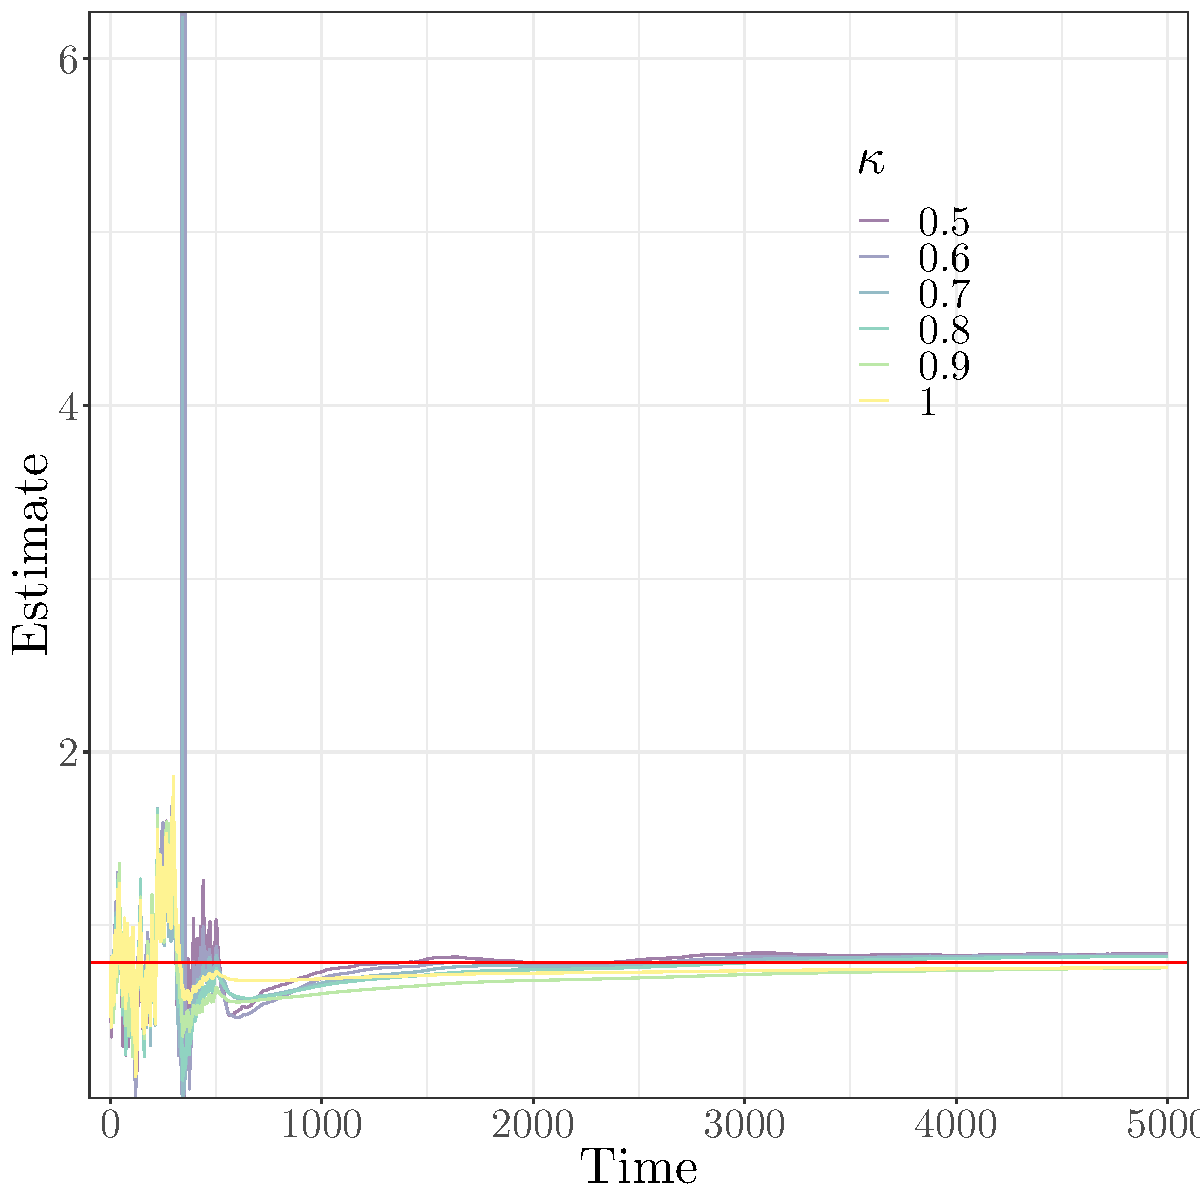
\includegraphics[width = 0.4\textwidth]{oneObs_oneStart_severalGrads_smooth.pdf}
\end{tabular}
\caption{\label{fig:1obs:1start:6Grads}(\textit{Left}) online estimation of $\theta$ for the data set presented in Figure \ref{fig:data}, with different decreasing rates values $\kappa$. (\textit{Right}) Averaged estimator, where $\hat{\parvec}$ is averaged after a burning phase of 300 time steps.}
\end{figure}




\begin{figure}
\begin{center}
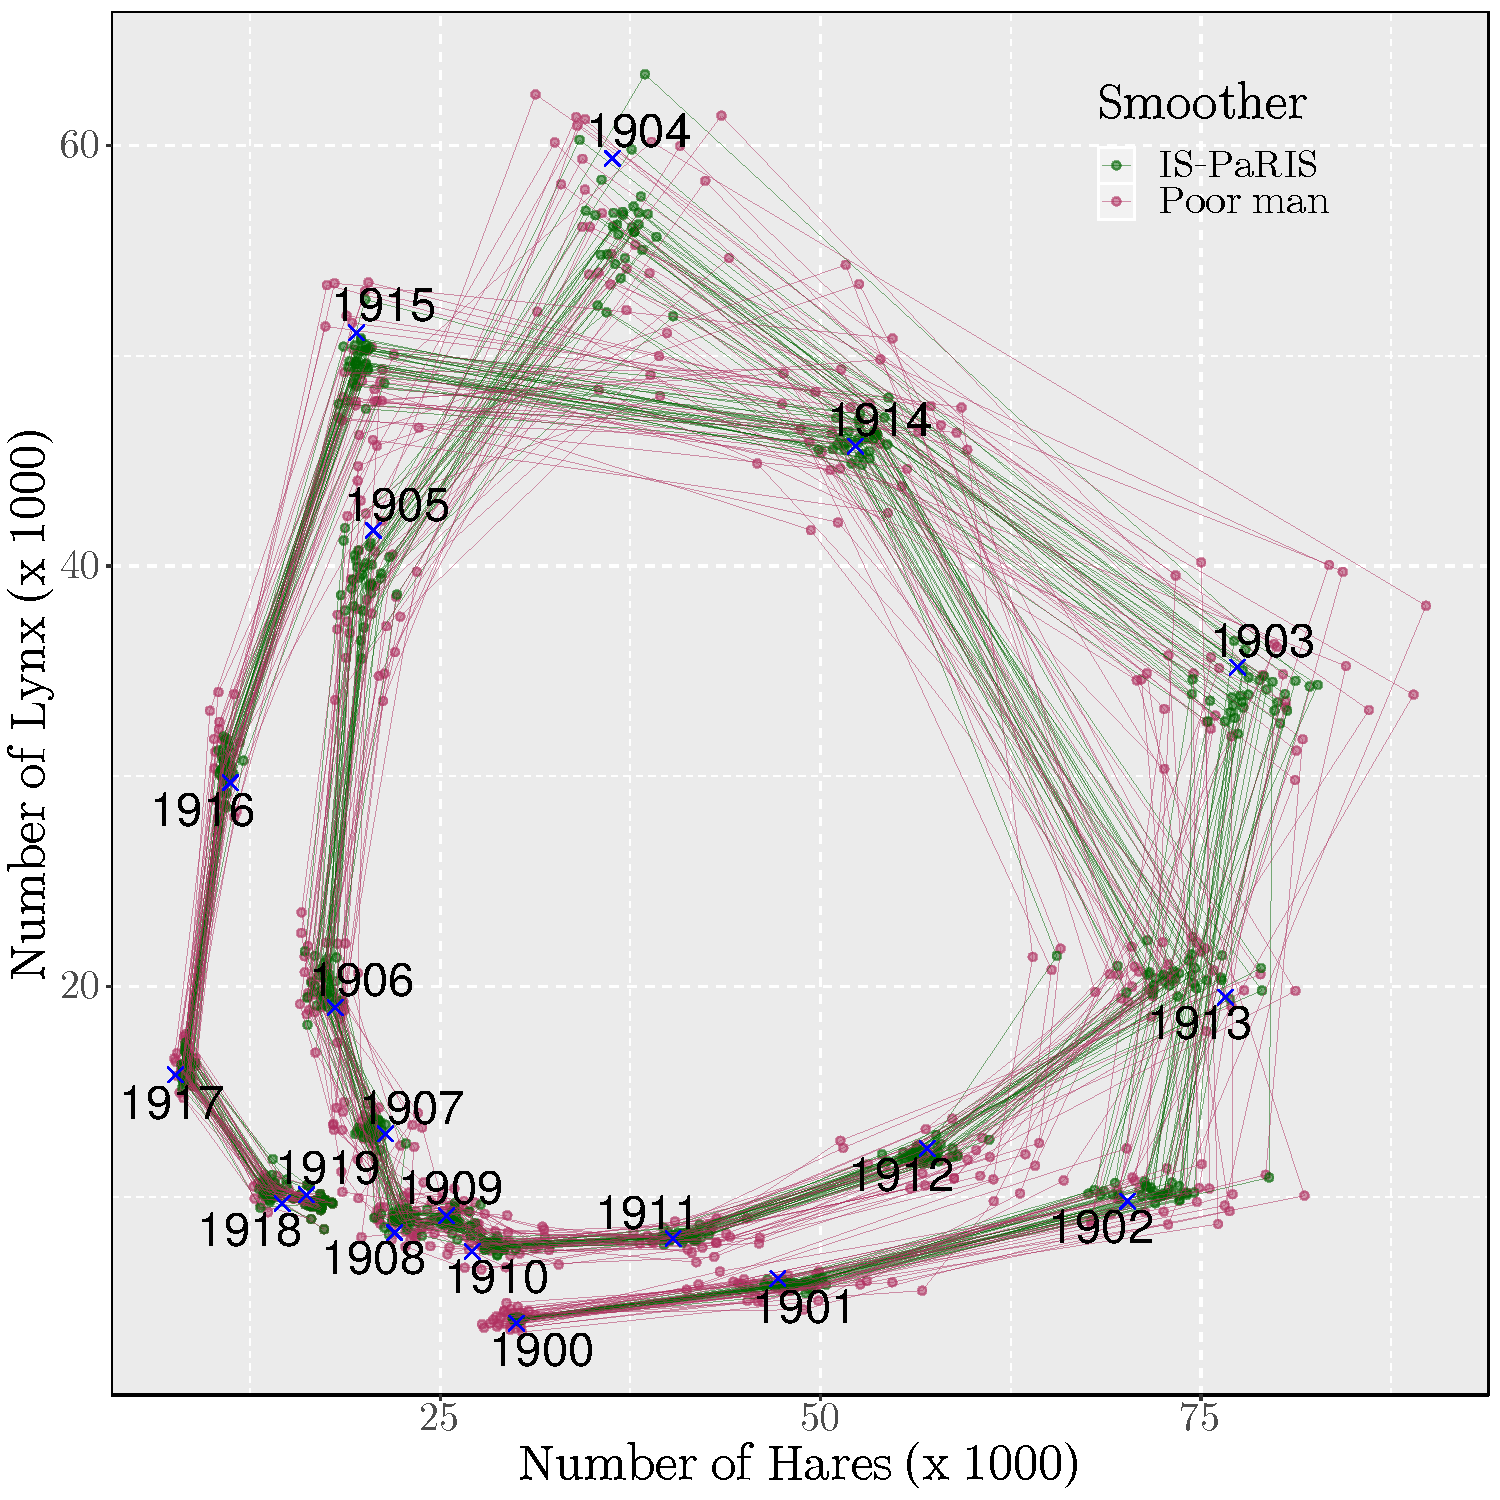
\includegraphics[scale = 0.4]{smoothing_hares_lynx.pdf}
\end{center}
\caption{\label{fig:LV:hares:lynx} Estimated Hares-Lynx abundances using the Hudson bay company data set. Both our IS-PaRIS smoother and the poor man smoother are performed to approximate the MLE and solve the tracking problem. Blue crosses show the observations.}
\end{figure}

\section{Discussion}
\label{sec:discussion} 
This paper proposes a solution to  perform online smoothing for latent data models with intractable transition densities and marginal conditional likelihood. This allows in particular to estimate smoothing expectations of additive functionals of solutions to generic SDEs.% i.e. obtaining a positive and almost surely bounded estimate of the transition density to run the  backward acceptance rejection mechanism. 

Note that the proposed backward importance sampling may be used to approximate expectations under the smoothing distributions for general state space hidden Markov models and  is not restricted to POD processes. As illustrated in various experiments, this approach may lead to significant  gains in computational time for similar performance than the acceptance rejection approach.  The proposed estimator, unlike the existing methods such as GPE-based algorithms, applies to a large range of multivariate diffusion processes (see \cite{andersson2017unbiased} and \cite{fearnhead2017continuous}).

Theoretical guarantees, such as consistency and asymptotic normality of this estimator remain to be proved. 
This should be an extension of \cite{gloaguen2021pseudo}; however, this would imply few technicalities which are out of the scope of this paper. The bias of the PaRIS algorithm may be shown to be or order $\mathcal{O}((1 + 1/\K)/\N)$ and vanishes as $\N$ goes to infinity for any choice of $\K\geqslant 2$. 
The exact sampling being replaced by an importance sampling step, the conjecture is that  the bias of the proposed algorithm involves a $\mathcal{O}(1/\K)$ term, which does not vanish as $\N$ goes to infinity. 
However, the empirical study illustrates that $\K$ may be chosen to increase with $\N$ sufficiently slowly to remove the additional bias term, while simultaneously ensuring better computational performance. % This empirical analysis could be supported by theoretical guarantees   and motivates future developments.

\bibliographystyle{apalike}
\bibliography{backwardIS}

\appendix 

\section{Application to partially observed SDE}
\label{sec:filter:SDE}
Let $(X_t)_{t\ge 0}$ be defined as a weak solution to the following Stochastic Differential Equation (SDE) in $\mathbb{R}^d$:
\begin{equation}
\label{eq:sde}
X_0 = x_0 \quad\mbox{and}\quad \rmd X_t = \alpha_{\parvec}(X_t)\rmd t + \rmd W_t\eqsp,
\end{equation}
where $(W_t)_{t\geqslant 0}$ is a standard Brownian motion, $\alpha_{\parvec}: \Xset\to\Xset$ is the drift function
% and $\Sigma_{\parvec}:\Xset\to\mathbb{R}^{2\dimX}$ is the diffusion
. The inference procedure presented in this paper is applied in the case where the solution to \eqref{eq:sde} is supposed to be partially observed at times $t_0 = 0,\ldots,t_n$, for a given $n\geqslant 1$, through an observation process $(Y_k)_{0\leqslant k \leqslant n}$ taking values in $\mathbb{R}^m$. For all $0\leqslant k \leqslant n$, the distribution of $Y_k$ given $(X_t)_{t\geqslant 0}$ depends on $X_k = X_{t_k}$ only and has density $\md{k;\parvec}$ with respect to $\nu$. The distribution of $X_0$ has density $\chi$ with respect to $\mu$ and for all $0\leqslant k \leqslant n-1$, the conditional distribution of $X_{k+1} $ given $(X_{t})_{0\leqslant t\leqslant k}$ has density $\hd{k+1;\parvec}(X_{k},\cdot)$ with respect to $\mu$. 
%This unknown density can be expressed as an expectation of a Brownian Bridge functional \cite{dacunha1986estimation}.
\subsection{Unbiased estimators of the transition densities}

The algorithm described above strongly relies on assumption H\ref{assum:unbiased}. 
In the context of SDEs, when $\md{k+1;\parvec}$ is available explicitly, this boils down to finding an unbiased estimate $\hdhat{k+1;\parvec}\langle \zeta\rangle(x,y)$ of $\hd{k+1;\parvec}(x,y)$ and defining
\[
\hatqg{k;\parvec}\langle \zeta\rangle(x,y) = \hdhat{k+1;\parvec}\langle \zeta\rangle(x,y)\md{k+1;\parvec}(x_{k+1},Y_{k+1})\eqsp.
\]

\subsection{General Poisson Estimators}
In \cite{olsson2011particle} and \cite{gloaguen2018online}, General Poisson Estimators (GPEs) are used to obtain an unbiased estimate of the transition density.  However, designing such estimators requires three strong assumptions \cite{beskos2006retrospective}.

\begin{enumerate}
\item The diffusion defined by \eqref{eq:sde} can be transformed into a unit diffusion through the Lamperti transform, with drift function $\tilde{\alpha}_\parvec(x)$.
\item The drift of this unit diffusion can be expressed as the gradient of a potential function, i.e., there exists a twice differentiable function $A_{\parvec}:\mathbb{R}^d \to \rset$ such $\tilde{\alpha}_{\parvec} = \nabla_x A_{\parvec}$.
\item The function $x\mapsto (\|\tilde{\alpha}_{\parvec}(x)\|^2 + \Delta A_{\parvec}(x))/2$ (where $\Delta$ denotes the Laplacian) is lower bounded.
\end{enumerate}

Assumption (1)
%(\ref{CIS:lamperti})
 is used to define a proposal distribution absolutely continuous with respect to the target which is easy to sample from. 
Assumption (2)
%(\ref{CIS:diffcoeff})
 is necessary to obtain a tractable Radon-Nikodym derivative between the proposal and the target distributions using the Girsanov transformation. 
 While these assumptions can be proved under mild assumptions for scalar diffusions, much stronger conditions are required in the multidimensional case \cite{ait-sahalia2008closed}. 

% for all $\parvec\in\parspace$, $\alpha_{\parvec}$ is of a gradient form $\alpha_{\parvec} = \nabla_x A_{\parvec}$ where $A_{\parvec}:\mathbb{R}^d \to \rset$ is a twice continuously differentiable function and that $x\mapsto (\|\alpha_{\parvec}(x)\|^2 + \Delta A_{\parvec}(x))/2$ is lower bounded by $\ell_{\parvec}$ where $\Delta$ is the Laplace operator. 
%By Girsanov theorem, for all $x$, $y$,
%\begin{multline*}
%%\label{eq:q:girsanov}
%\hd{k+1;\parvec}(x,y) = \varphi_{\Delta_k}(x-y)\mathrm{e}^{A_{\parvec}(y) - A_{\parvec}(x) - \ell(\parvec)\Delta_k}\\
%\pE_{\mathbb{W}_x^{\Delta_k,y}}\left[\mathrm{exp}\left(-\int_0^{\Delta_k} \psi_{\parvec}(\omega_s)\rmd s\right)\right]\eqsp,
%\end{multline*}
%where $\psi_{\parvec}: x \mapsto (\|\alpha_{\parvec}(x)\|^2 + \Delta A_{\parvec}(x))/2 - \ell_{\parvec}$, $\Delta_k = t_{k+1}-t_k$, for all $a>0$, $\varphi_a$ is the probability density function of a centered Gaussian random variable with variance $a$ and for all $t>0$, $\mathbb{W}_x^{t,y}$ is the law of Brownian bridge starting at 0 at time 0 and ending at $y$ at time $t$. 
%Assume that there exist random variables $L_W$ and $U_W$ such that for all $0\leqslant s \leqslant \Delta_k$, $L_W \leqslant \psi_{\parvec}(\omega_s) \leqslant U_W$. Let $\kappa$ be a random variable taking values in $\mathbb{N}$ with distribution $\mu$, $\omega = (\omega_s)_{0 \leq s \leq t}$ be the realization of a Brownian Bridge with distribution  $\mathbb{W}_x^{t,y}$, and $(U_j)_{1\leqslant j \leqslant \kappa}$ be independent uniform random
%variables on $(0,\Delta_k)$ and $\zeta = (\kappa,\omega, U_1, \ldots , U_{\kappa})$. As
%shown in \cite{fearnhead2008particle}, the Girsanov transform leads to a positive unbiased estimator given by
%\begin{multline*}
%\hdhat{k+1;\parvec}(x,y;\zeta) = \varphi_{\Delta_k}(x-y)\mathrm{e}^{A_{\parvec}(y) - A_{\parvec}(x) - L_W\Delta_k}\\
%\times \prod_{j=1}^{\kappa}\frac{U_W-\varphi_{\parvec}(\omega_{{U_j}})}{U_W-L_W}
%\end{multline*}
%and
%\[
%\hatqg{k;\parvec}(x,y;\zeta) = \hdhat{k+1;\parvec}(x,y;\zeta)\md{k+1;\parvec}(x_{k+1},Y_{k+1})\eqsp.
%\]
Let $\omega = (\omega_s)_{0 \leq s \leq t}$ be the realization of a Brownian Bridge starting at $x$ at time 0 and ending in $y$ at time $\Delta$. The distribution of $\omega$ is denoted by  $\mathbb{W}_x^{\Delta,y}$. 
Moreover, suppose that for all $\parvec\in\parspace$, $\alpha_{\parvec}$ is of a gradient form $\alpha_{\parvec} = \nabla_x A_{\parvec}$ where $A_{\parvec}:\Xset \to \rset$ is a twice continuously differentiable function. Denoting, $ \psi_\theta:~~x \mapsto  \psi_\theta(x) = (\|\alpha_{\parvec}(x)\|^2 + \Delta A_{\parvec}(x))/2$, by Girsanov theorem, for all $x, y \in \mathbb{R}^d \times \mathbb{R}^d$
\begin{equation}
\label{eq:q:girsanov}
\hd{k+1;\parvec}(x,y) = \phi_{\Delta_k}(x-y)\mathrm{exp}\left(A_{\parvec}(y) - A_{\parvec}(x)\right)\mathbb{E}_{\mathbb{W}_x^{\Delta_k,y}}\left[\mathrm{exp}\left(-\int_0^{\Delta_k} \psi_{\parvec}(\omega_s)\rmd s\right)\right]\eqsp,
\end{equation}
where $\Delta_k = t_{k+1}-t_k$, for all $a>0$, $\phi_a$ is the probability density function of a centered Gaussian random variable with variance $a$. The transition density then cannot be computed as it involves an integration over the whole path between $x$ and $y$. 
To perform the algorithm proposed in this paper, we therefore have to design a positive an unbiased estimator of $\hd{k+1;\parvec}(x,y)$. 

\paragraph{Unbiased GPE estimator for $\hd{k+1;\parvec}(x,y;\zeta)$.}

Assume that there exist random variables $\gpeLB$ and $\gpeUB$ such that for all $0\leqslant s \leqslant \Delta_k$, $\gpeLB \leqslant \psi_{\parvec}(\omega_s) \leqslant \gpeUB$. Let $\kappa$ be a random variable taking values in $\mathbb{N}$ with distribution $\mu$, $\omega = (\omega_s)_{0 \leq s \leq \Delta_k}$ be the realization of a Brownian Bridge, and $(U_j)_{1\leqslant j \leqslant \kappa}$ be independent uniform random
variables on $(0,\Delta_k)$ and $\zeta = (\kappa,\omega, U_1, \ldots , U_{\kappa})$. As
shown in \cite{fearnhead:papaspiliopoulos:roberts:2008}, equation \eqref{eq:q:girsanov} leads to a positive unbiased estimator given by
\[
\hdhat{k+1;\parvec}(x,y;\zeta) = \phi_{\Delta_k}(x-y)\mathrm{exp}\left(A_{\parvec}(y) - A_{\parvec}(x) - \gpeLB\Delta_k\right)\prod_{j=1}^{\kappa}\frac{\gpeUB-\psi_{\parvec}(\omega_{{U_j}})}{\gpeUB-\gpeLB}\eqsp.
\]

\paragraph{Unbiased GPE estimator of $\nabla_{\parvec}\log\hd{k+1;\parvec}(x,y)$.}
Let's denote $\varphi_{\parvec}:~x \mapsto \psi_{\parvec}(x) - \gpeLB$. 
By \eqref{eq:q:girsanov},
\begin{multline*}
\nabla_{\parvec}\log\hd{k+1;\parvec}(x,y) = \nabla_{\parvec}A_{\parvec}(y) - \nabla_{\parvec}A_{\parvec}(x) - \nabla_{\parvec}\gpeLB \Delta_k\\
-\frac{\mathbb{E}_{\mathbb{W}_x^{\Delta_k,y}}\left[\left(\int_0^{\Delta_k} \nabla_{\parvec}\varphi_{\parvec}(\omega_s)\rmd s\right)\mathrm{exp}\left(-\int_0^{\Delta_k} \varphi_{\parvec}(\omega_s)\rmd s\right)\right]}{\mathbb{E}_{\mathbb{W}_x^{\Delta_k,y}}\left[\mathrm{exp}\left(-\int_0^{\Delta_k} \varphi_{\parvec}(\omega_s)\rmd s\right)\right]}\eqsp.
\end{multline*}
 On the other hand, the diffusion bridge $\mathbb{S}^{\Delta_k,y}_{\parvec,x}$ associated with the SDE \eqref{eq:sde} is absolutely continuous with respect to $\mathbb{W}_x^{\Delta_k,y}$ with Radon-Nikodym derivative given by
\begin{align*}
\frac{\rmd \mathbb{S}^{\Delta_k,y}_{\parvec,x}}{\rmd \mathbb{W}_x^{\Delta_k,y}}(\omega) &= \left[\hd{k+1;\parvec}(x,y)\right]^{-1}\phi_{\Delta_k}(x-y)\mathrm{exp}\left(A_{\parvec}(y) - A_{\parvec}(x) - \gpeLB\Delta_k-\int_0^{\Delta_k} \varphi_{\parvec}(\omega_s)\rmd s\right)\eqsp,\\
&=\mathbb{E}_{\mathbb{W}_x^{\Delta_k,y}}\left[\mathrm{exp}\left(-\int_0^{\Delta_k} \varphi_{\parvec}(\omega_s)\rmd s\right)\right]^{-1}\mathrm{exp}\left(-\int_0^{\Delta_k} \varphi_{\parvec}(\omega_s)\rmd s\right)\eqsp.
\end{align*}
This yields
\[
\nabla_{\parvec}\log\hd{k+1;\parvec}(x,y) = \left(\nabla_{\parvec}A_{\parvec}(y) - \nabla_{\parvec}A_{\parvec}(x) - \nabla_{\parvec}\gpeLB\Delta_k\right) - \mathbb{E}_{\mathbb{S}_{\parvec,x}^{\Delta_k,y}} \left[\int_0^{\Delta_k} \nabla_{\parvec}\varphi_{\parvec}(\omega_s)\rmd s\right]
\]
and an unbiased estimator of $\nabla_{\parvec}\log\hd{k+1;\parvec}(x,y)$ is given by
\[
\mathsf{l}_{k+1;\parvec}(x,y,\mathsf{s}^{\parvec,x,y,\Delta_k}_U) = \left(\nabla_{\parvec}A_{\parvec}(y) - \nabla_{\parvec}A_{\parvec}(x) - \nabla_{\parvec}\gpeLB\Delta_k\right) - \Delta_k\nabla_{\parvec}\varphi_{\parvec}(\mathsf{s}^{\parvec,x,y,\Delta_k}_U)\eqsp,
\]
where $U$ is uniform on $(0,1)$ and independent of $\mathsf{s}^{\parvec,x,y,\Delta_k}\sim \mathbb{S}_{\parvec,x}^{\Delta_k,y}$. In the context of GPE, $\mathsf{s}^{\parvec,x,y,\Delta_k}$ can be simulated exactly using exact algorithms for diffusion processes proposed in \cite{beskos2006retrospective}.


\subsection{Parametrix estimators}

More recently, \cite{andersson2017unbiased} and \cite{fearnhead2017continuous} proposed an algorithm which can be used under weaker assumptions. 
This parametrix algorithm draws weighted skeletons using an importance sampling mechanism for diffusion processes. 
In this case, the sampled paths are not distributed as the target process but the weighted samples produce unbiased estimates of expectations of functionals of this process. To obtain an unbiased estimator $\hdhat{k+1}\langle \zeta\rangle(x,y)$, the parametrix algorithm draws weighted skeletons at random times $s_0 = 0 < s_1<\dots<s_j $, denoted by $\left\{(x_{s_j},\mathsf{w}_{s_j})\right\}_{j\geqslant 0}$, where $x_0 = x$ and $\mathsf{w}_0=1$. 
The update times $(s_j)_{j\geqslant 0}$ are instances of an inhomogeneous Poisson process of intensity $\lambda(t)$. 
Let $(x_{s_j},\mathsf{w}_{s_j})$ be the last weighted sample and $s_{j+1}$ be the next update time of the trajectory.  While $s_{j+1}<\Delta t_{k}$, the new state is sampled using a simple Euler scheme, namely:
\begin{align*}
x_{s_{j+1}} &\eqdef x_{s_j} + \Delta s_j\alpha_{\parvec}(x_{s_j}) + (\Delta s_j)^{1/2}\sigma_{\parvec}(x_{s_j})\varepsilon_{j+1}\eqsp,
\end{align*}
where $\Delta s_j \eqdef s_{j+1}-s_j$, $\Delta t_{k} = t_{k+1} - t_{k}$ and $\varepsilon_{j+1}\sim\mathcal{N}_d(0,I_d)$. 
The proposal density associated with this procedure is denoted by $m_{j;\parvec}\left(x_{s_j},\cdot,\Delta\tau_j\right)$. 
Let $\mathcal{K}^{\parvec}$ (resp. $\mathcal{K}^{j,\parvec}_{\mathrm{prop}}$) denote the Kolmogorov forward operator of the diffusion  (resp. the Kolmogorov forward operator of the proposal distribution $m_{j;\parvec}\left(x_{s_j},\cdot,\Delta s_j
\right)$). 
The forward operators write, for any function $h:\mathbb{R}^d\rightarrow\mathbb{R}$,
$$
\mathcal{K}^{\theta}h\left(y\right) \eqdef -\sum_{i=1}^d\frac{\partial}{\partial y_i}\left\{\alpha_{\parvec,i}(y)h\left(y\right)\right\} + \sum_{i,\ell=1}^d\frac{1}{2}\frac{\partial^2}{\partial y_i\partial y_\ell}\left\{\gamma_{\parvec,i,\ell}(y)h\left(y\right)\right\}\eqsp,
$$
where $\gamma_\parvec = \sigma_\parvec \sigma_\parvec^T$.
Then, following \cite{fearnhead2017continuous}, the weight is updated by
\[
\mathsf{w}_{s_{j+1}}\eqdef\mathsf{w}_{s_j}\rho^{\lambda}_j\left(x_{s_j},x_{s_{j+1}},\Delta s_j\right)\eqsp,
\]
where
\begin{equation}
\label{CIS:eq:rho}
\rho^{\lambda}_j\left(x,y,u\right)\eqdef 1+\frac{\left(\mathcal{K}-\mathcal{K}^{j,\theta}_{\mathrm{prop}}\right)m_{j;\parvec}\left(x,z,u\right)_{|z=y}}{\lambda(u)m_{j;\parvec}\left(x,y,u\right)}\eqsp.
\end{equation}
It is worth noting that \eqref{CIS:eq:rho} can be computed using only first derivatives of $\alpha_{\parvec}$ and second derivatives of $\sigma_\parvec$. 
If $N_k$ is the number of Poisson events between $0$ and $\Delta t_{k}$, the parametrix unbiased estimate is then given by 
\[
\hdhat{k+1}\langle \zeta_k\rangle(x,y) = \mathsf{w}_{s_{N_k}}m_{k;\parvec}\left(x_{s_{N_k}},y,t_{k+1} - s_{N_k}\right) \eqsp,
\]
where $\zeta_k$ stands for all the randomness required to produce the parametrix estimator (Poisson process and Gaussian random variables).

The stability of this estimator is studied in \cite{fearnhead2017continuous} which provides $\mathrm{L}_p$ controls for the weight $\mathsf{w}_{s_{N_k}}$. 
The parametrix algorithm mentioned above is a highly flexible procedure to obtain such an unbiased estimate for a much broader class of diffusions than Poisson based estimations which require strong assumptions. 
However, as the update \eqref{CIS:eq:rho} involves the difference of two Kolmogorov operators, the parametrix estimator of the transition density may be negative, and has no reason to satisfy \eqref{eq:AR:bound}.
Thus, the SMC algorithms described above cannot be implemented.



%Moreover, maximum likelihood estimation of $\theta$ requires an unbiased estimator of $\nabla_{\parvec}\log\hd{k+1;\parvec}(x,y)$. 
%Such two estimators can be obtained using the General Poisson Estimator (GPE, \cite{fearnhead:papaspiliopoulos:roberts:2008}).



\end{document}
